% =============================================================================
% GREEDY BORUTA - ECML-PKDD SUBMISSION WIREFRAME
% =============================================================================
% Format: Springer LNCS (Lecture Notes in Computer Science)
% Max length: 16 pages including references (Research Track)
% Review: Double-blind
% =============================================================================

%Nicolas, algumas observacoes sobre o paper:

% 1 - Introduzimos o conceito de weakly and strongly confirmed features. Isso tem impacto no output da biblitoca greedy boruta, mas nao tem muito impacto no paper em si.

% 2 - Introduzimos a analise de FPR pra quando o numero de shadows eh r <= p. Eu nao mexi nas secoes de resultados do paper, porque todas as secoes usam p shadow features. No entanto, eu criei uma nova secao (e esta vazia) no apendice B onde podemos colocar resultados do GB usando r shadow features versus o vanilla boruta e o GB com p shadow features. Estava pensando em pegar os datasets os 4 datasets com os maiores numeros de features e meio que escrever uma secao bem resumida dos resultados no estilo da secao q esta no paper. O q acha? Se achar interessante, compartilha os arquivos que geram os resultados da secao de dados reais que eu me viro.

% 3 - Estava pensando em mover a secao "Reducing the Number of Shadow Features" pro Apendice B. A ideia eh legal, mas nao sei se faz tanto sentido deixar essa secao no meio do paper. Me diz o que vc acha.

% 4 - Eu fiz varias alteracoes, algumas maiores e outras menores. Dessa vez eu nao aceitei, entao o paper ta cheio que alteracoes pra vc ver onde eu mexi exatamente.

% 5 - Remover o titulo “Undecidedness & …” da figura 5. A legenda ja diz a mesma coisa.

% Idem pra Figura 4. A legenda e o titulo dizem a mesma coisa.

% Remover o titutlo “Ground-Truth metrics by alpha” da figura 2.

% 6 - Pra mandarmos pro Chris, so preciso que vc de uma olhada no paper e resolva os comentarios. Todos os pontos acima podem ser resolvido apos o envio do paper ao Chris, pq ele nao vai conseguir ler o paper de imediato. 

\documentclass[runningheads]{llncs}

% =============================================================================
% PACKAGES
% =============================================================================
\usepackage{graphicx}
\let\proof\relax
\let\endproof\relax
\usepackage{amsthm}
\usepackage{amsmath,amssymb}
\usepackage{esvect}
\usepackage{algorithm}
\usepackage{algorithmic}
\usepackage{booktabs}
\usepackage{multirow}
\usepackage{xcolor}
\usepackage{hyphenat}
\usepackage{subcaption}
\usepackage{xurl}
\usepackage{hyperref}
\usepackage{cleveref}
\usepackage{microtype}

% \usepackage[htt]{hyphenat}
% DRAFT ONLY: forces figures to appear exactly where declared in source (no floating).
% TO REVERT FOR SUBMISSION: remove the float package import below and change all
% \begin{figure}[H] back to \begin{figure}[H] (or [htbp] for more placement flexibility).
\usepackage{float}
% DRAFT ONLY: cap figure height so images don't fill an entire page and leave blank gaps.
% TO REVERT FOR SUBMISSION: remove the two \setlength lines below, and remove the
% height=... keepaspectratio arguments from each \includegraphics call in section 5.
\setlength{\abovecaptionskip}{4pt}
\setlength{\belowcaptionskip}{0pt}

% For wireframe TODO notes - REMOVE BEFORE SUBMISSION
\usepackage[colorinlistoftodos,textsize=small]{todonotes}
\newcommand{\writeme}[1]{\todo[inline,color=yellow!40]{WRITE: #1}}
\newcommand{\addcite}[1]{\todo[inline,color=blue!20]{CITE: #1}}
\newcommand{\addfigure}[1]{\todo[inline,color=green!20]{FIGURE: #1}}
\newcommand{\addtable}[1]{\todo[inline,color=orange!20]{TABLE: #1}}
\newcommand{\decision}[1]{\todo[inline,color=red!20]{DECISION: #1}}

\newtheorem{assumption}{Assumption}

% =============================================================================
% TITLE AND AUTHORS
% =============================================================================
\begin{document}

\title{Trading statistical conservatism for speed: A `greedy' modification to Boruta}
% Alternative titles:
% - Trading Statistical Conservatism for Speed: A Greedy Modification to Boruta
% - Fast All-Relevant Feature Selection with Provable Guarantees

\titlerunning{Greedy Boruta}

% For double-blind submission, use anonymous authors
% \author{Anonymous}
% \author{}
% \authorrunning{Anonymous}
% \institute{Anonymous Institution}

% For camera-ready version, uncomment and fill:
\author{Nicolas Vana \and Estevão Prado}
\authorrunning{Vana and Prado}
\institute{Bradesco Bank, São Paulo, Brazil}
% \email{nicolas.v.santos@bradesco.com.br}
% \email{nicolas.vana@bradesco.com.br}
% \and Institution 2, City, Country}

\maketitle

% =============================================================================
% ABSTRACT (~150-200 words)
% =============================================================================

\begin{abstract}
The Boruta algorithm is the most widely adopted method for all-relevant feature selection, but its computational cost and lack of convergence guarantees limit its applicability in modern high-dimensional settings, where the number of features $p$ frequently exceeds $10^4$. We propose Greedy Boruta, a modification that replaces Vanilla Boruta's binomial confirmation test with a single-hit rule: a feature is confirmed if it ever exceeds the maximum shadow importance in any iteration. Despite its simplicity, this change yields four formal guarantees: convergence in exactly $K = \lceil \log_2(p/\alpha) \rceil$ iterations, feature recall at least as high as Vanilla Boruta when both methods observe the same importance scores and use the same rejection test, simplification of the final BH rejection calculation and a per-feature false positive rate bounded above by $K/(p+1)$, which decreases as dimensionality grows. The deterministic iteration count eliminates all termination-related hyperparameters and enables embarrassingly parallel execution, implemented in \texttt{greedyboruta} (available on PyPI). We further introduce a weak/strong confirmation framework that distinguishes features satisfying the original Boruta confirmation criterion from those selected exclusively by the greedy criterion, providing users with an interpretable measure of confidence among the confirmed features. We also show that the number of shadow features can be reduced from \(p\) to \(r \leq p\), yielding an explicit trade-off between computational cost and false positive control. On a synthetic benchmark with known ground truth and six real-world high-dimensional datasets, Greedy Boruta achieves 1.8 to 66.2 times speedups while detecting no statistically significant difference in downstream model performance relative to Vanilla Boruta in $15$ of the $18$ benchmark configurations.

\keywords{Feature selection \and Boruta algorithm \and All-relevant features \and Computational efficiency \and Parallelization}
\end{abstract}



\section{Introduction}
\label{sec:introduction}

Feature selection is a critical preprocessing step in high-dimensional machine learning pipelines, reducing computational cost, improving model interpretability and mitigating overfitting. Methods for feature selection broadly fall into two paradigms. \emph{Minimal-optimal} methods, such as Lasso~\cite{tibshirani1996lasso}, Ridge~\cite{hoerl1970ridge}, Recursive Feature Elimination~\cite{guyon2002rfe} and mRMR~\cite{peng2005mrmr}, seek the smallest subset of features that maximizes predictive performance. \emph{All-relevant} methods instead aim to identify every feature that carries information about the target variable, regardless of redundancy. The all-relevant paradigm is particularly valuable in scientific discovery~\cite{rak2019evaluation}, biomarker identification~\cite{mardian2023ovarian} and causal inference~\cite{pellet2008markov}, where discarding a relevant feature represents a permanent loss of information that no downstream analysis can recover, even if there is redundancy between features.

The Boruta algorithm~\cite{kursa2010feature,kursa2010boruta} is the most widely adopted method for all-relevant feature selection. Its statistical framework, based on comparing each feature's importance against permuted ``shadow'' copies that represent the maximum achievable importance by random noise, provides a principled mechanism for distinguishing signal from noise. Since its introduction, Boruta has been adopted across diverse domains including bioinformatics~\cite{rak2019evaluation,mardian2023ovarian}, finance~\cite{pinto2024forecasting,li2024stock} and natural language processing~\cite{sallah2024fake,tan2024mosquito}, and several variants have been proposed. For instance, BorutaPy~\cite{borutapy} offers an equivalent Python implementation to the original R implementation, while BorutaSHAP~\cite{borutashap} replaces impurity-based importance with SHAP-value~\cite{lundberg2017shap} based importances. However, none of the available variants address two fundamental limitations of the algorithm. 

First, Boruta is computationally expensive. Each iteration requires training a tree-based ensemble on a dataset augmented with $p$ shadow features, and the algorithm may require hundreds or thousands of iterations to resolve all features. In modern industrial and scientific applications where $p$ is often in the thousands, running Boruta to completion can require days of computation, making the method impractical in time-constrained settings. Second, Boruta provides no convergence guarantees (the state in which all features are either confirmed or rejected). That is, features can remain \emph{tentative}, neither confirmed nor rejected, forcing practitioners to either increase the iteration budget arbitrarily, enable heuristic early stopping mechanisms or resolve remaining tentatives using post-hoc heuristics such as the rough fix~\cite{kursa2010feature}. In practice, this uncertainty requires careful tuning of hyperparameters that control the maximum number of iterations and early-stopping, creating a tension between computational cost and quality of the solution.
etermines the tota
% In this paper, we propose Greedy Boruta, a modification that replaces Boruta's binomial test confirmation criterion with a single-hit rule: a feature is confirmed if it ever exceeds the maximum shadow importance in any iteration. This change is motivated by the fact that, in the all-relevant paradigm, false negatives (missed relevant features) are costlier than false positives (incorrectly included noise features), since false positives can be filtered out by downstream regularization, cross-validation or minimal-optimal selection methods. Despite its simplicity, this modification yields theoretical and computational properties, namely: guaranteed convergence in few iterations, provably equal or higher feature recall (i.e., true positive rate) than Vanilla Boruta, embarrassingly parallel execution, simplification of multiple-testing corrections and elimination of all termination-related hyperparameters. Throughout this paper, we refer to the original algorithm and its equivalent reimplementations collectively as \emph{Vanilla Boruta}, and to our proposed modification as \emph{Greedy Boruta}.

In this paper, we propose Greedy Boruta, a modification that replaces Boruta's binomial-test confirmation criterion with a single-hit rule: a feature is confirmed if it exceeds the maximum shadow importance in at least one iteration. This change is motivated by the fact that, under the all-relevant paradigm, false negatives (missed relevant features) are often more costly than false positives (incorrectly included noise features), since false positives can be filtered by downstream regularization, cross-validation, stability analyses or minimal-optimal feature selection procedures. We further introduce two practical extensions. First, we partition confirmed features into \emph{strongly confirmed} and \emph{weakly confirmed} groups. Strongly confirmed features satisfy the original Boruta confirmation criterion and therefore would also be selected by Vanilla Boruta, whereas weakly confirmed features are selected exclusively by Greedy Boruta and may be viewed as additional candidate variables for further investigation. Second, we show that the number of shadow features can be reduced from $p$ to $r \leq p$, substantially decreasing the dimensionality of the augmented dataset and yielding further computational savings in high-dimensional settings. Throughout this paper, we refer to the original algorithm and its equivalent reimplementations collectively as \emph{Vanilla Boruta}, and to our proposed modification as \emph{Greedy Boruta}.

\medskip 
The main contributions of this paper are:
\begin{enumerate}
    \item \textbf{Algorithmic:} A modification to Boruta that guarantees convergence in exactly $K = \lceil \log_2(p/\alpha) \rceil$ iterations\footnote{\label{fn:bonf}Under Bonferroni correction.}, eliminating all termination-related hyperparameters. We further introduce a weak/strong confirmation framework that distinguishes features satisfying the original Boruta confirmation criterion from those selected exclusively by the greedy criterion.
    \item \textbf{Theoretical:} Proofs of (i) a recall guarantee showing that the set of selected features by Vanilla Boruta is contained in the set of features selected by Greedy Boruta (Theorem~\ref{thm:recall}), (ii) a convergence bound on the number of iterations (Theorem~\ref{thm:convergence}), (iii) simplification of the final Benjamini--Hochberg rejection calculation (Corollary~\ref{cor:bh}), (iv) a false positive rate (FPR) upper bound of $K/(p+1)$ (Theorem~\ref{thm:fpr}) and (v) an analysis of the effect of reducing the number of shadow features from \(p\) to \(r \leq p\) on the computational and statistical properties of Greedy Boruta.
    \item \textbf{Practical:} A reduced-shadow variant of Greedy Boruta that decreases the dimensionality of the augmented dataset from \(2p\) to \(p+r\), yielding additional computational savings while allowing practitioners to explicitly control the trade-off between runtime and false positive rate. The deterministic iteration count and independence across iterations enable embarrassingly parallel execution, implemented in the \texttt{greedyboruta} PyPI package.
    \item \textbf{Practical:} The \texttt{greedyboruta} package, available on PyPI, provides a Python implementation of Greedy Boruta. This implementation includes a reduced-shadow  parameter that uses \(r \leq p\) shadow features, reducing the dimensionality of the augmented dataset from \(2p\) to \(p+r\) and offering a tunable trade-off between computational cost and the bound on the per-feature false positive rate. 
\end{enumerate}


\section{Background: The Boruta Algorithm}
\label{sec:background}

The idea behind Vanilla Boruta is to construct \emph{shadow features}, permuted copies of features that serve as competitive benchmarks to the non-shadow features. By comparing each non-shadow feature's importance against the maximum shadow importance across multiple randomized trials, Boruta makes statistically principled decisions about which features carry genuine signal and which are not statistically distinguishable from noise.

The algorithm operates iteratively, with each iteration consisting of four steps.
\begin{enumerate}
    \item \textbf{Shadow feature construction}: for each of the $p$ original features, Boruta creates a shadow copy by randomly permuting the feature's values across samples. This permutation destroys any relationship with the target variable while preserving the feature's marginal distribution. The dataset is then extended to include both the $p$ original features and $p$ shadow features. 
    \item \textbf{Importance scoring}: a tree-based ensemble (originally random forests~\cite{breiman2001random}) is trained on this extended dataset, and feature importance scores are extracted for all $2p$ features. 
    \item \textbf{Hit registration}: each original feature whose importance exceeds the maximum shadow importance in that iteration receives a `hit', and these hits are accumulated across iterations. 
    \item \textbf{Statistical testing}: binomial tests determine whether the features are confirmed (relevant), tentative (unknown) or rejected (irrelevant).
\end{enumerate}

The statistical testing framework employs two one-sided binomial tests at each iteration. For a feature with $h$ hits across $K$ iterations, the confirmation test checks whether $\mathbb{P}(X \geq h \mid K, \theta=0.5) \leq \alpha$, where $\alpha$ denotes statistical significance and $p = 0.5$ represents the null hypothesis that the feature is no better than random noise (represented by the best shadow). The symmetric rejection test checks $\mathbb{P}(X \leq h \mid K, \theta=0.5) \leq \alpha$. Both tests are typically applied with a feature-wise Bonferroni correction to control the family-wise error rate across the $p$ features under test. Features passing neither test remain tentative. In both the R and Python implementations, these tests are repeated at every iteration (in \texttt{boruta\_py}, from the fifth iteration onward) and decisions are final: only tentative features are re-tested, and rejected features are removed from all subsequent iterations.

Because there are no convergence guarantees with Vanilla Boruta, when the algorithm terminates with tentative features unresolved, whether by early stopping or reaching a maximum number of iterations, features that remain tentative are resolved using the rough fix heuristic \cite{kursa2010feature}. Under this heuristic, a tentative feature is confirmed if its median importance across iterations exceeds the median of the per-iteration maximum shadow importances, and rejected otherwise. 

The use of artificial variables as negative controls also underlies knockoff methods~\cite{barber2015controlling,candes2018panning}. However, model-X knockoffs are designed to control the false discovery rate, whereas Boruta targets all-relevant feature selection through comparisons with permuted shadow features. Knockoff guarantees also rely on an exchangeability property of the joint distribution of original and knockoff covariates that permuted shadow features do not generally satisfy; the exchangeability assumption used in our analysis (Section~\ref{sec:method:fpr}) concerns only the importance scores. Another related approach, PIMP~\cite{altmann2010permutation}, calibrates feature importance against null distributions estimated by repeatedly permuting the response.

\section{The Greedy Boruta Algorithm}
\label{sec:method}

% We now present Greedy Boruta, a modification of Vanilla Boruta that achieves dramatic computational speedups while maintaining theoretical guarantees on feature recall. The asymmetry between false negatives (missed relevant features) and false positives (incorrectly confirmed noise features) discussed in Section~\ref{sec:introduction} motivates a relaxation of the confirmation criterion: rather than requiring statistically significant evidence that a feature consistently outperforms random noise, we confirm a feature upon the first indication that it carries signal. This change yields convergence in exactly $K = \lceil \log_2(p/\alpha) \rceil$ iterations (with Bonferroni correction) or $K = \lceil \log_2(1/\alpha) \rceil$ iterations (without), eliminates the need for hyperparameters governing termination, enables embarrassingly parallel execution and, under the conditions of Theorem~\ref{thm:recall}, selects every feature that Vanilla Boruta would confirm.

Motivated by the asymmetry between false negatives and false positives discussed in Section~\ref{sec:introduction}, Greedy Boruta replaces Vanilla Boruta's binomial confirmation test with a single-hit rule: a feature is confirmed if its importance exceeds the maximum shadow importance in at least one iteration. The rejection criterion is retained, but "evaluated" only after a predetermined number of iterations.

Algorithm~\ref{alg:greedy_boruta} presents the complete Greedy Boruta procedure. Given a dataset with $p$ features and a target variable $y$, the algorithm first determines the total required number of iterations $K$, which depends on the number of features and significance level. At each iteration, shadow features are generated by randomly permuting the values of every original feature, thereby preserving marginal distributions while destroying any association with the target. A tree-based ensemble model is then trained on the augmented dataset containing both original and shadow features, and feature importance scores are computed. The maximum importance score among the shadow features defines a noise threshold for that iteration. Any original feature whose importance exceeds this threshold receives a hit. After all iterations are completed, features with at least one hit are confirmed as relevant, whereas features with zero hits are rejected.

The key difference relative to Vanilla Boruta lies in the confirmation step, while the rejection criterion remains effectively unchanged. Vanilla Boruta employs sequential binomial hypothesis tests to determine whether a feature should be confirmed or rejected, whereas Greedy Boruta confirms any feature that achieves at least one hit across all iterations. This modification appears in lines~$14$ and~$15$ of Algorithm~\ref{alg:greedy_boruta}, where the greedy confirmation rule replaces the statistical confirmation test. Furthermore, because a feature with zero hits never exceeds the maximum shadow importance in any iteration, rejection can be determined directly at the end of the procedure without repeatedly performing intermediate statistical tests. Consequently, Greedy Boruta eliminates the sequential testing mechanism used in Vanilla Boruta, resulting in a simpler and more computationally efficient algorithm while preserving the same underlying principle of comparing real features against randomized shadow features.

\begin{algorithm}[t]
\caption{Greedy Boruta Algorithm}
\label{alg:greedy_boruta}
\begin{algorithmic}[1]
\REQUIRE Dataset $X \in \mathbb{R}^{n \times p}$, target $y$, significance level $\alpha$
\ENSURE Set of confirmed features $\mathcal{C}$, rejected features $\mathcal{R}$
\STATE Compute $K = \lceil \log_2(p/\alpha) \rceil$ \COMMENT{Total iterations}
\STATE Initialize $\text{hits}[j] = 0$ for all features $j = 1, \ldots, p$
\FOR{$i = 1$ to $K$}
    \STATE Create shadow features by permuting each column of $X$
    \STATE Train tree ensemble on $[X, X_{\text{shadow}}]$ with target $y$
    \STATE Compute importance scores for all features
    \STATE $m \gets \max(\text{importance of shadow features})$
    \FOR{each original feature $j$}
        \IF{$\text{importance}[j] > m$}
            \STATE $\text{hits}[j] \gets \text{hits}[j] + 1$
        \ENDIF
    \ENDFOR
\ENDFOR
\STATE $\mathcal{C} \gets \{j : \text{hits}[j] \geq 1\}$ \COMMENT{Greedy confirmation}
\STATE $\mathcal{R} \gets \{j : \text{hits}[j] = 0\}$ \COMMENT{All others rejected ($\text{p-value} \leq \alpha/p$)} 
\RETURN $\mathcal{C}, \mathcal{R}$
\end{algorithmic}
\end{algorithm}

% We point out that shadow features used by Vanilla Boruta and Greedy Boruta are conceptually related to the knockoff variables introduced by \cite{barber2015controlling,candes2018panning}. In both approaches, artificial variables are constructed to serve as negative controls against which the importance of the original features can be assessed. Our exchangeability assumption, which is formally introduced in Section \ref{sec:method:fpr} and under which an irrelevant feature and the shadow features are equally likely to attain the maximum importance, is closely related to the exchangeability property that underpins the theoretical guarantees of the model-X knockoff framework. Despite this conceptual similarity, the objectives of the two methodologies differ substantially. Model-X knockoffs are designed to control the false discovery rate under assumptions on the joint distribution of the covariates, whereas Boruta and Greedy Boruta target the all-relevant feature selection problem by comparing feature importances with randomly permuted shadow variables. Greedy Boruta therefore should be viewed as a modification of the Boruta algorithm rather than as an alternative to knockoff-based inference. We also note that permutation-based importance calibration methods, such as PIMP~\cite{altmann2010permutation}, pursue a related objective by estimating the null distribution of feature importance scores through repeated permutations, but likewise address a different inferential problem.

\subsection{Weak and strong confirmations}

A potential limitation of the Greedy Boruta confirmation rule is that all features with at least one hit are treated equally, regardless of the total number of hits accumulated across iterations. In particular, a feature that beats the shadow threshold once receives the same confirmation status as a feature that consistently outperforms the shadow threshold. To provide a more nuanced interpretation of the selected features while preserving the feature recall guarantee established in Theorem~\ref{thm:recall}, which is presented in Section \ref{sec:method:theory}, we propose partitioning the confirmed features into \emph{strongly} and \emph{weakly} confirmed groups.

Let \(H_j\) denote the number of hits accumulated by feature \(j\) after \(K\) iterations. Recall that Greedy Boruta confirms a feature whenever \(H_j \geq 1\). Define the set of confirmed features as
\[
\mathcal{C}_G
=
\{j : H_j \geq 1\}.
\]
We further define the set of \emph{strongly confirmed} features as
\[
\mathcal{C}_{\mathrm{strong}}
=
\left\{
j :
\mathbb{P}\!\left(
X \geq H_j
\right)
\leq \alpha/p,
\quad
X \sim \mathsf{Binomial}(K,\theta = 0.5)
\right\}.
\]
That is, a feature is strongly confirmed if it satisfies the original Boruta confirmation criterion under the Bonferroni correction. Equivalently, these are the features that would be confirmed by Vanilla Boruta after \(K\) iterations. 

The remaining confirmed features are classified as \emph{weakly confirmed} and are part of the set
\[
\mathcal{C}_{\mathrm{weak}}
=
\left\{
j :
H_j \geq 1
\ \text{and}\
\mathbb{P}\!\left(
X \geq H_j
\right)
>
\alpha/p,
\quad
X \sim \mathsf{Binomial}(K,\theta = 0.5)
\right\}.
\]
The distinction between weak and strong confirmations provides a natural ranking of the selected features. Strongly confirmed features have accumulated sufficient evidence to satisfy the original Boruta significance criterion and therefore correspond to features that would also be selected by Vanilla Boruta. In contrast, weakly confirmed features are selected exclusively by Greedy Boruta. These features have demonstrated some evidence of relevance by outperforming the shadow threshold at least once, but the evidence is not strong enough to achieve statistical significance under the Boruta binomial test.

From a practical perspective, strongly confirmed features may be interpreted as high-confidence discoveries, whereas weakly confirmed features may warrant additional investigation through domain expertise, stability analyses or downstream predictive validation. This distinction allows Greedy Boruta to retain its computational advantages and feature recall guarantee while providing users with a measure of confidence among the selected features.

\subsection{Theoretical Properties}
\label{sec:method:theory}

% RESTRUCTURE: overview paragraphs removed; their content was merged into the theorem subsections below
% (Maintained Recall -> 3.2.1; Guaranteed Convergence + Hyperparameter Simplification -> 3.2.2;
% Parallelization -> new subsection "Parallel Execution" after Multiple Testing Corrections).
% \paragraph{Maintained Recall.}
% Greedy Boruta confirms a feature after a single hit, whereas Vanilla Boruta requires a statistically significant number of hits. Theorem~\ref{thm:recall} shows that, as a result, every feature confirmed by Vanilla Boruta is also confirmed by Greedy Boruta ($\mathcal{C}_V \subseteq \mathcal{C}_G$), so Greedy Boruta's feature recall is never lower. This guarantee holds run by run when both methods observe the same importance scores through iteration $K$ and Vanilla Boruta permanently rejects every zero-hit feature at that iteration. Under these conditions, any feature that Vanilla Boruta eventually confirms must have obtained at least one hit within the first $K$ iterations, which is exactly Greedy Boruta's confirmation rule.
% \paragraph{Guaranteed Convergence.}
% As we prove in Theorem~\ref{thm:convergence}, the greedy criterion allows computing \emph{a priori} the exact number of iterations required for convergence, solving the uncertain termination of Vanilla Boruta. Notably, the minimum number of iterations for Vanilla Boruta to make its first confirmation or rejection in a given task equals the total iteration count at which Greedy Boruta completes for that same task.
% \paragraph{Hyperparameter Simplification.}
% A direct consequence of the guaranteed convergence is a hyperparameter simplification in the implementation of Greedy Boruta. Namely, the \texttt{max\_iter} (maximum number of Boruta iterations), \texttt{early\_stopping} (heuristic stopping rule), and \texttt{n\_iter\_no\_change} (how many consecutive iterations with no change in feature status are tolerated) parameters present in the \texttt{boruta\_py} package are not required.

We now state the theoretical guarantees of Greedy Boruta. Full proofs are provided in Appendix~\ref{app:proofs}.

\subsubsection{Feature Recall Guarantee}

Our first result shows that relaxing the confirmation criterion never costs recall relative to Vanilla Boruta.

\begin{theorem}[Feature Recall Guarantee]
\label{thm:recall}
% Consider a common realization in which Vanilla Boruta and Greedy Boruta share the same feature and maximum-shadow importance scores through iteration $K$. Greedy Boruta terminates at $K$, while Vanilla Boruta terminates at any finite iteration $T\geq K$. Assume Vanilla applies the matched non-strict rejection test by iteration $K$, rejecting every still-tentative feature with zero hits by then, and that rejections are final, as in the R and Python implementations, which drop rejected features from all later iterations. Let \(\mathcal{C}_V\) and \(\mathcal{C}_G\) denote the sets of features confirmed by Vanilla Boruta and Greedy Boruta, respectively, using the same significance level and correction setting. Then,
% $$
% \mathcal{C}_V \subseteq \mathcal{C}_G.
% $$
% The inclusion holds regardless of whether Vanilla Boruta confirms a feature through the binomial test or through the rough-fix heuristic applied to tentative features at termination.
Suppose Vanilla Boruta, as described in Section~\ref{sec:background}, and Greedy Boruta use the same significance level and correction setting and observe the same feature and maximum-shadow importance scores through iteration $K$, and that Vanilla Boruta runs for at least $K$ iterations. Let $\mathcal{C}_V$ and $\mathcal{C}_G$ denote the sets of features they confirm. Then $\mathcal{C}_V \subseteq \mathcal{C}_G$, whether Vanilla Boruta confirms a feature through the binomial test or through the rough fix.
\end{theorem}

% The key insight is that both confirmation mechanisms in Vanilla Boruta (the binomial test and the rough fix) require a feature to have at least one hit. For the binomial test, zero hits yield a p-value of 1, which cannot be rejected. For the rough fix, a feature with zero hits has its empirical importance distribution stochastically dominated \cite{levy1990stochastic} by the maximum shadow importance, so its median cannot exceed the shadow median. Since the greedy criterion confirms any feature with at least one hit, every feature confirmed by Vanilla Boruta is also confirmed by Greedy Boruta.
The result follows because Greedy Boruta's confirmation rule is the weakest possible: a single hit. A feature with no hits in the first $K$ iterations cannot be confirmed by Vanilla Boruta's binomial test, since its confirmation p-value is 1, and because Vanilla Boruta applies the same rejection test at iteration $K$, it is rejected there. Because rejections are final, the rough fix, which only acts on tentative features, cannot confirm it later either. Every feature Vanilla Boruta confirms therefore has at least one hit by iteration $K$, which is exactly Greedy Boruta's confirmation rule. Consequently, Greedy Boruta's feature recall is never lower than Vanilla Boruta's.

% Two implementation settings fall outside the conditions of Theorem~\ref{thm:recall}. First, the \texttt{two\_step=True} mode of \texttt{boruta\_py} adds a trial-wise correction that makes rejection at iteration $K$ harder, so a zero-hit feature is not guaranteed to be rejected there. Second, the R implementation uses strict inequalities ($<\alpha$ rather than $\leq\alpha$). This changes the rejection decision at iteration $K$ only when $p/\alpha$ (or $1/\alpha$, without Bonferroni correction) is an exact power of two, which cannot happen for the usual choices $\alpha = 10^{-m}$ or $\alpha = 0.05$.

\subsubsection{Convergence Guarantee}

Unlike Vanilla Boruta, whose number of required iterations cannot be known in advance, Greedy Boruta runs for a fixed number of iterations that is sufficient to resolve every feature.

\begin{theorem}[Convergence Guarantee]
\label{thm:convergence}
% Here, convergence means that no features remain tentative. For a dataset with $p$ features, Algorithm~\ref{alg:greedy_boruta} uses a predetermined budget of exactly $K = \lceil \log_2(p/\alpha) \rceil$ iterations when using Bonferroni correction for multiple comparisons, after which every feature is classified as confirmed or rejected.
Consider a dataset with $p$ features, and let $\alpha$ be the significance level of the binomial rejection test. With Bonferroni correction, after $K = \lceil \log_2(p/\alpha) \rceil$ iterations of Algorithm~\ref{alg:greedy_boruta}, every feature is either confirmed or rejected, so no feature remains tentative.
\end{theorem}

At iteration $K$, every feature with at least 1 hit is confirmed by the greedy criterion. Every remaining feature has zero hits and thus a rejection p-value of $(0.5)^K$. Under Bonferroni correction, rejection requires $(0.5)^K \leq \alpha/p$, which holds by construction of $K = \lceil \log_2(p/\alpha) \rceil$. Therefore, all features are classified and the algorithm terminates. It is worth noting that the number of iterations decomposes as $K = \lceil \log_2(p) + \log_2(1/\alpha) \rceil$: halving $\alpha$ or doubling $p$ adds exactly one iteration. Table~\ref{tab:iterations_alpha} shows $K$ for representative values.

\begin{table}[H]
\centering
\caption{Number of iterations $K = \lceil \log_2(p/\alpha) \rceil$ required for convergence when using Bonferroni correction for multiple comparisons.}
\label{tab:iterations_alpha}
\begin{tabular}{c|ccccc}
\toprule
& \multicolumn{5}{c}{Number of features $p$} \\
$\alpha$ & 50 & 100 & 500 & 1000 & 5000 \\
\midrule
0.100 & 9 & 10 & 13 & 14 & 16 \\
0.050 & 10 & 11 & 14 & 15 & 17 \\
0.010 & 13 & 14 & 16 & 17 & 19 \\
0.001 & 16 & 17 & 19 & 20 & 23 \\
$10^{-4}$ & 19 & 20 & 23 & 24 & 26 \\
$10^{-5}$ & 23 & 24 & 26 & 27 & 29 \\
\bottomrule
\end{tabular}
\end{table}

\noindent Without Bonferroni correction (analogous to \texttt{mcAdj=FALSE} in the R implementation), the iteration count reduces to $K = \lceil \log_2(1/\alpha) \rceil$, and the number of iterations is not dependent on the number of features anymore. In Sections \ref{sec:experiments:setup} and \ref{sec:experiments:realworld}, we use the Bonferroni correction to obtain $K$.

The same bound also limits Vanilla Boruta: with fewer than $K$ iterations, no binomial test can reach significance, so Vanilla Boruta cannot confirm or reject any feature before iteration $K$. Greedy Boruta therefore finishes at the earliest iteration at which Vanilla Boruta can make its first decision. Because the iteration count is known in advance, the termination-related parameters of \texttt{boruta\_py} (\texttt{max\_iter}, \texttt{early\_stopping} and \texttt{n\_iter\_no\_change}) are no longer needed.

\paragraph{Parallel execution.}
\label{sec:method:parallel}
Because the iteration budget $K$ is fixed in advance (Theorem~\ref{thm:convergence}) and no features are removed during execution, every iteration uses the same feature set and differs only in its random seed. The iterations are therefore independent: each produces a vector of hits, and the final hit counts are their sum. All $K$ iterations can run in parallel, and their results only need to be combined at the final classification step. Vanilla Boruta cannot be parallelized this way, because each iteration depends on the previous ones: rejected features are dropped, the binomial tests are re-evaluated after every iteration and early stopping tracks consecutive iterations without change. \texttt{greedyboruta} implements this iteration-level parallelism with \texttt{joblib}; its practical benefit depends on the base estimator's own parallelism, as discussed in Section~\ref{sec:experiments:setup}.

% RESTRUCTURE: the BH result was moved from its own subsubsection (3.2.3) into Multiple Testing Corrections below and turned into a corollary.
% \subsubsection{Simplification of the Final BH Rejection Calculation}
% The result below concerns the Benjamini--Hochberg calculation for rejecting zero-hit features. It does not establish FDR control among greedily confirmed features: their selection bypasses this test. The per-feature FPR bound in Section~\ref{sec:method:fpr} and FDR among selected features are distinct quantities.
% \begin{theorem}[BH Rejection Simplification]
% At iteration $K$ in Greedy Boruta, all tentative features (those with 0 hits) have identical p-values equal to $(0.5)^K$. Consequently, the Benjamini-Hochberg FDR correction \cite{benjamini1995controlling} either rejects all tentative features or none, making the correction equivalent to an uncorrected test.
% \end{theorem}
% This follows directly from the greedy confirmation criterion: all features with at least 1 hit are already confirmed, so the only features entering the rejection test have exactly zero hits and identical p-values. The Benjamini-Hochberg procedure \cite{benjamini1995controlling} applied to a set of identical p-values reduces to a single threshold comparison. This contrasts with Vanilla Boruta, where tentative features accumulate different hit counts and thus have a distribution of p-values, making FDR correction non-trivial.

\subsection{Multiple Testing Corrections}
\label{sec:method:corrections}

% Table~\ref{tab:correction_mapping} summarizes how the correction settings in \texttt{greedyboruta} relate to those available in the most widely used Boruta implementations. In Vanilla Boruta, multiple-testing correction is required both across features and across iterations because confirmation and rejection decisions are repeatedly revisited throughout the execution of the algorithm. In contrast, Greedy Boruta performs a single rejection test at the final iteration and does not rely on hypothesis testing for confirmation. Consequently, trial-wise correction becomes unnecessary. Furthermore, by Corollary~\ref{cor:bh}, FDR-based procedures reduce to the uncorrected test. As a result, the only non-trivial correction remaining in Greedy Boruta is the feature-wise Bonferroni adjustment, controlled through the \texttt{bonferroni} parameter.

In Vanilla Boruta, multiple-testing correction is required both across features and across iterations, because confirmation and rejection decisions are revisited at every iteration. Greedy Boruta performs a single rejection test at the final iteration and does not use a hypothesis test for confirmation, so trial-wise correction becomes unnecessary. The following corollary of Theorem~\ref{thm:convergence} shows that FDR correction becomes unnecessary as well.

\begin{corollary}[BH Rejection Simplification]
\label{cor:bh}
At iteration $K$, every feature not confirmed by Greedy Boruta has zero hits and therefore the same rejection p-value $2^{-K}$. The Benjamini--Hochberg procedure~\cite{benjamini1995controlling} applied to these features rejects all of them, exactly as the uncorrected test does.
\end{corollary}

Applied to a set of identical p-values, the Benjamini--Hochberg procedure reduces to comparing their common value with $\alpha$, and $2^{-K}\leq\alpha$ holds under either correction setting. In Vanilla Boruta, by contrast, tentative features have different hit counts and therefore different p-values, so FDR correction is not trivial there. Note that Corollary~\ref{cor:bh} concerns only the rejection of zero-hit features. It does not establish FDR control among the confirmed features, since greedy confirmation bypasses this test; false positives among confirmed features are analysed in Section~\ref{sec:method:fpr}. As a result, the only non-trivial correction remaining in Greedy Boruta is the feature-wise Bonferroni adjustment, controlled through the \texttt{bonferroni} parameter. Table~\ref{tab:correction_mapping} maps this setting to its equivalents in the most widely used Boruta implementations.

\begin{table}[t]
\centering
\caption{Mapping between correction settings across implementations.}
\label{tab:correction_mapping}
\begin{tabular}{lll}
\toprule
\texttt{greedyboruta} & R Boruta & \texttt{boruta\_py} \\
\midrule
\texttt{bonferroni=True}  & \texttt{mcAdj=TRUE}  & \texttt{two\_step=False} \\
\texttt{bonferroni=False} & \texttt{mcAdj=FALSE} & \texttt{two\_step=True}\footnotemark \\
\bottomrule
\end{tabular}
\end{table}

\footnotetext{The \texttt{two\_step=True} mode applies both FDR and trial-wise Bonferroni correction; both degenerate in Greedy Boruta (Corollary~\ref{cor:bh}), reducing to the uncorrected case.}

% RESTRUCTURE: the "Parallel Execution" subsection was turned into a run-in \paragraph at the end of the Convergence Guarantee subsubsection.

\subsection{False Positive Rate Analysis}
\label{sec:method:fpr}

The feature recall and convergence guarantees come at a cost: by relaxing the confirmation criterion, Greedy Boruta may confirm features that Vanilla Boruta would leave tentative or reject. We quantify this trade-off under a standard assumption of the Boruta framework.

\begin{assumption}[Shadow Exchangeability]
\label{asm:exchangeability}
An irrelevant feature is exchangeable with the shadow features with respect to the importance measure. That is, the importance of an irrelevant feature and the importances of the $p$ shadow features are identically distributed and symmetric under permutation within each iteration.
\end{assumption}

% Moved (shortened) to the knockoff paragraph in Section 2 (Background):
% This assumption concerns exchangeability among importance scores. It is distinct from the model-X knockoff requirement that the joint distribution of original and knockoff covariates remain invariant under swaps of corresponding variables \cite{candes2018panning}; randomly permuted shadow features do not generally satisfy that requirement.

Violations of this assumption (e.g., importance measure biases toward high-cardinality features~\cite{strobl2007bias,altmann2010permutation}) can affect both Vanilla Boruta and Greedy Boruta, since both use the same shadow mechanism. Their different decision rules can nevertheless respond differently to these violations. The analysis below isolates the effect of the modified decision rule under the stated assumption.

Under the shadow exchangeability assumption, the importance of an irrelevant feature and the $p$ shadow importances form $p+1$ exchangeable random variables. Each has the same probability of being the unique maximum, so the per-iteration hit probability satisfies $\theta_0 \leq 1/(p+1)$. Equality holds when the maximum is unique almost surely; ties can reduce the probability of strictly exceeding all shadows.

\begin{theorem}[FPR of Greedy Boruta]
\label{thm:fpr}
% Under Assumption~\ref{asm:exchangeability} in each iteration, the probability that Greedy Boruta falsely confirms an irrelevant feature satisfies
% \begin{equation}
%     \mathbb{P}(\text{false positive}) \leq \sum_{i=1}^{K}\mathbb{P}\!\left(I_j^{(i)} > M^{(i)}\right) \leq \frac{K}{p+1},
% \end{equation}
% where $K = \lceil \log_2(p/\alpha) \rceil$. This quantity is bounded above by
% \begin{equation}
%     \mathbb{P}(\text{false positive}) \leq \frac{K}{p + 1} = \frac{\lceil \log_2(p/\alpha) \rceil}{p + 1}.
% \end{equation}
% If there are $m_0$ irrelevant features, linearity of expectation gives $\mathbb{E}[\mathrm{FP}]=\sum_{j\in\mathcal{N}}\mathbb{P}(j\text{ is confirmed})\leq m_0 K/(p+1)$, where $\mathcal{N}$ is the set of irrelevant features. Independence between features is not required. Consequently, $\mathbb{E}[\mathrm{FP}]/p\leq (m_0/p)K/(p+1)$ bounds false positives relative to the original number of features; it does not bound their proportion among selected features.
Suppose Assumption~\ref{asm:exchangeability} holds in every iteration, and let $K = \lceil \log_2(p/\alpha) \rceil$. Then, for any irrelevant feature $j$,
\begin{equation}
\label{eq:fpr_bound}
    \mathbb{P}(j \text{ is confirmed by Greedy Boruta}) \leq \frac{K}{p + 1} = \frac{\lceil \log_2(p/\alpha) \rceil}{p + 1}.
\end{equation}
Consequently, if $m_0$ of the $p$ features are irrelevant, the expected number of false positives satisfies $\mathbb{E}[\mathrm{FP}] \leq m_0 K/(p+1)$.
\end{theorem}

% The proof, given in Appendix~\ref{app:proofs}, uses the union bound and does not require independence across iterations. If the hit events are additionally independent across iterations and the maximum is unique almost surely, the exact probability is $1-(p/(p+1))^K$.
The proof, given in Appendix~\ref{app:proofs}, applies a union bound over the $K$ iterations: an irrelevant feature is falsely confirmed if it obtains a hit in at least one iteration, and each iteration contributes a hit probability of at most $1/(p+1)$. The bound on $\mathbb{E}[\mathrm{FP}]$ then follows by summing over the irrelevant features (linearity of expectation). Neither step requires independence, so the result holds even when iterations are dependent or irrelevant features are correlated. Note that $\mathbb{E}[\mathrm{FP}]$ counts false positives; it does not bound their proportion among the selected features (the FDR), which also depends on how many relevant features are confirmed.

The bound is also close to the exact value in an idealized setting. If hits in different iterations were independent and ties impossible, an irrelevant feature would miss in all $K$ iterations with probability $(p/(p+1))^K$, so it would be falsely confirmed with probability exactly $1-(p/(p+1))^K$. For $p=500$ and $\alpha=0.05$, this is $2.76\%$, against the bound of $2.79\%$.

The bound also has a favorable structure: the numerator grows logarithmically while the denominator grows linearly, so the FPR \emph{decreases} as $p$ increases. Table~\ref{tab:fpr} presents the bound for representative configurations. For moderate to large $p$ (the typical Boruta use case), the bound is small: at most $5.2\%$ for $p = 500$ and below $3\%$ for $p \geq 1{,}000$ across all $\alpha$ values shown. For small $p$ (e.g., $p = 100$), the bound can exceed $10\%$, but in such settings the computational cost of Vanilla Boruta is typically manageable.

\begin{table}[t]
\caption{Upper bound on per-feature false positive rate (FPR) of Greedy Boruta under Bonferroni correction ($K = \lceil \log_2(p/\alpha) \rceil$). Each cell shows the value of the bound in Equation~\eqref{eq:fpr_bound}.}
\label{tab:fpr}
\centering
\begin{tabular}{c|cc|cc|cc|cc}
\toprule
& \multicolumn{2}{c|}{$p = 100$}
& \multicolumn{2}{c|}{$p = 500$}
& \multicolumn{2}{c|}{$p = 1{,}000$}
& \multicolumn{2}{c}{$p = 10{,}000$} \\
$\alpha$
& $K$ & FPR
& $K$ & FPR
& $K$ & FPR
& $K$ & FPR \\
\midrule
$0.05$    
& 11 & $10.89\%$
& 14 & $2.79\%$
& 15 & $1.50\%$
& 18 & $0.18\%$ \\

$0.01$    
& 14 & $13.86\%$
& 16 & $3.19\%$
& 17 & $1.70\%$
& 20 & $0.20\%$ \\

$0.001$   
& 17 & $16.83\%$
& 19 & $3.79\%$
& 20 & $2.00\%$
& 24 & $0.24\%$ \\

$0.0001$  
& 20 & $19.80\%$
& 23 & $4.59\%$
& 24 & $2.40\%$
& 27 & $0.27\%$ \\

$0.00001$ 
& 24 & $23.76\%$
& 26 & $5.19\%$
& 27 & $2.70\%$
& 30 & $0.30\%$ \\
\bottomrule
\end{tabular}
\end{table}

The same analysis naturally extends to the case where only $r \leq p$ shadow features are generated at each iteration. Under Assumption~\ref{asm:exchangeability}, the per-iteration hit probability of an irrelevant feature becomes $\theta_0^\star \leq 1/(r+1)$, yielding the corresponding upper bound $\mathbb{P}(\mathrm{FP}) \leq K/(r+1)$. Although reducing the number of shadow features weakens false positive control, it decreases the dimensionality of the augmented dataset from $2p$ to $p+r$, providing additional computational and memory savings. This reduction in shadow dimensionality may be particularly relevant in distributed computing environments such as Apache Spark \cite{zaharia2016spark}, where constructing and materializing shadow features may become a bottleneck. A detailed theoretical analysis of this reduced-shadow variant, together with empirical results illustrating the resulting computational--statistical trade-off, is presented in Appendix~\ref{app:add_results_reducing_shadows}.

% REVISION NOTE: Numerical results and figures below predate the corrected fold-local evaluation.
% Rerun publication_benchmark.py and regenerate them before submission; NI margins must be prespecified.
% \section{Experimental Evaluation}
% \label{sec:experiments}
 
% We evaluate Greedy Boruta on two complementary fronts. First, using a synthetic dataset with a known ground truth, we measure selection quality directly against the true relevant feature set across a sweep of significance levels~$\alpha$ and analyse how Vanilla Boruta's quality evolves over iterations relative to the point at which Greedy Boruta terminates by design. Second, we validate on a suite of real-world high-dimensional benchmarks where ground truth is
% unavailable, using downstream model performance as a proxy for selection quality. We point out that all experiments in this section use the original Boruta setting with $p$ shadow features. Results for the reduced-shadow variant ($r \leq p$) of Greedy Boruta, which explicitly trades false positive control for additional computational savings, are presented in Appendix~\ref{app:add_results_reducing_shadows}.

% We compare Greedy Boruta primarily against the R implementation's default configuration (\texttt{mcAdj=TRUE}, applying feature-wise Bonferroni correction). In practice, since the comparison is made with the \texttt{boruta\_py} package, we use \texttt{two\_step=False} to match the R defaults. All experiments use $R=10$ independent random seeds; results are reported as mean~$\pm$~standard deviation (std) unless stated otherwise.
 
% % -----------------------------------------------------------------------------
% \subsection{Synthetic Dataset Experiments}
% \label{sec:experiments:setup}
 
% We construct a controlled synthetic benchmark using \texttt{sklearn.datasets.make\_classification} with the following parameters: $n=1{,}000$ samples, $p=500$ features (\texttt{n\_informative = 5}, \texttt{n\_redundant = 100}, \texttt{n\_repeated = 0}, remaining $m_0 = 395$ are pure noise), one cluster per class (\texttt{n\_clusters\_per\_class = 1}), a low class separation (\texttt{class\_sep = 0.0001}) to prevent trivial discrimination, and a 30\% label noise rate (\texttt{flip\_y = 0.3}). All features are standardized to zero mean and unit variance prior to selection. Because the Boruta algorithm is designed for the all-relevant paradigm, we consider both the 5 informative and the 100 redundant features as relevant. We call this set of 105 relevant features the \emph{Broad}~GT (ground truth). The significance level is swept over $\alpha \in \{10^{-5},\,10^{-4},\,10^{-3},\,10^{-2},\,10^{-1}\}$. The base estimator for both methods is \texttt{ExtraTreesClassifier}~\cite{geurts2006extremely,pedregosa2011scikit}(\texttt{max\_depth=5}, \texttt{n\_estimators=`auto'}, \texttt{n\_jobs=-1}). Vanilla Boruta is configured with \texttt{max\_iter=512}, \texttt{early\_stopping=True} (\texttt{n\_iter\_no\_change=128}), and \texttt{two\_step=False}. Greedy Boruta uses Bonferroni correction (\texttt{bonferroni=True}) and \texttt{n\_jobs=4} for outer iteration-level parallelism. All experiments were run on an Intel Core~i7-14700K (3.40~GHz, 20 cores: 8P+12E), and with 64~GB RAM.

% \paragraph{Parallelism and speedup decomposition.}
% Both methods use the same base estimator configuration with \texttt{n\_jobs=-1}. Vanilla Boruta executes its iterations sequentially; Greedy Boruta additionally distributes iterations across 4 workers, parallelizing iterations as well as tree construction. Consequently, the observed speedup possibly reflects two factors: (i)~fewer iterations ($K = \lceil \log_2(p/\alpha) \rceil$ vs.\ hundreds) and (ii)~outer iteration-level parallelism. However, because each base estimator training call already saturates most of the available cores, effect (i) dominates (ii) in terms of speedup in most cases. Realistically, in non-cluster environments, the marginal benefit of outer parallelism is sub-linear and substantially smaller than the iteration-count reduction.

% \paragraph{Performance Metrics.}
% We evaluate against Broad~GT using four feature-level binary classification metrics: recall ($\text{TP}/(\text{TP}+\text{FN})$), precision ($\text{TP}/(\text{TP}+\text{FP})$), specificity ($\text{TN}/(\text{TN}+\text{FP})$) and F1 score ($\text{2*TP}/(\text{2*TP}+\text{FP}+\text{FN})$), where a \emph{true positive} (TP) is a relevant feature that was confirmed, a \emph{false positive} (FP) is a noise feature incorrectly confirmed, a \emph{false negative} (FN) is a relevant feature missed and a \emph{true negative} (TN) is a noise feature correctly rejected. Runtime comparisons use wall-clock time in seconds and speedup is defined as the ratio of each Vanilla Boruta run's time to the Greedy Boruta time.
 
% \begin{figure}
%     \centering
%     \includegraphics[width=\textwidth, height=0.8\textheight, keepaspectratio]{alpha_effect_boxplots.png}
%     \caption{Final-state ground-truth metrics across significance levels ($\alpha$) for Vanilla
%     Boruta and Greedy Boruta on the synthetic dataset. Individual runs are shown as semi-transparent dots; markers with caps show mean $\pm$ SE.}
%     \label{fig:final_state_metrics}
% \end{figure}
 
% Figure~\ref{fig:final_state_metrics} shows the final-state metric distributions. Greedy Boruta achieves equal or higher feature recall than Vanilla Boruta at every $\alpha$ level, in line with Theorem~\ref{thm:recall}. The cost is a modest reduction in precision and specificity: across individual runs, Greedy Boruta incorrectly confirms between 4 and 11 noise features (out of 395), a small fraction of the noise space. Recall is statistically greater for Greedy Boruta (one-sided Welch $t$-test, $p < 0.01$) and precision and specificity are statistically smaller at all $\alpha$ levels, as expected. No statistically significant difference in F1 was detected between the two methods at any $\alpha$ level (two-sided Welch $t$-test, $p > 0.01$), consistent with the competing effects of higher recall and lower precision offsetting each other. Mean speedup ratios (Figure~\ref{fig:final_state_metrics}, bottom panel) fall within the range of 20--35$\times$ across all $\alpha$ values.
 
% \subsection{Real-World Benchmarks}
% \label{sec:experiments:realworld}
 
% To validate Greedy Boruta beyond controlled synthetic settings, we evaluate it on six publicly available high-dimensional benchmark datasets spanning both classification and regression tasks (Table~\ref{tab:realworld_datasets}). Unlike the synthetic setting described in Section~\ref{sec:experiments}, the ground-truth relevant feature sets are unknown for these datasets, preventing direct evaluation of feature-selection accuracy. We therefore assess selection quality indirectly through downstream predictive performance. Both Greedy Boruta and Vanilla Boruta are executed independently using the same base estimator (\texttt{ExtraTreesClassifier} or \texttt{ExtraTreesRegressor}), parallelism configuration and hardware environment. After each method selects its subset of relevant features, a downstream Light Gradient Boosting Machine (LightGBM) model~\cite{ke2017lightgbm} is trained using only the selected features. Performance is then evaluated using 5-fold cross-validation and measured by weighted F1 score (classification) and $R^2$ (regression).

% %Each (dataset, $\alpha$, method) configuration is repeated over $R = 10$ independent random seeds; results are reported as mean~$\pm$~SE.
 
% \begin{table}
% \centering
% \caption{Real-world benchmark datasets.}
% \label{tab:realworld_datasets}
% \begin{tabular}{llrrll}
% \toprule
% Dataset    & Domain          & $n$    & $p$      & Task           & Source \\
% \midrule
% Madelon    & Artificial      & 2{,}000  & 500      & Classification & \cite{guyon2004result} \\
% Gisette    & Digit recog.    & 6{,}000  & 5{,}000  & Classification & \cite{guyon2004result} \\
% Arcene     & Mass spectrom.  & 100      & 10{,}000 & Classification & \cite{guyon2004result} \\
% Dexter     & Text classif.   & 300      & 20{,}000 & Classification & \cite{guyon2004result} \\
% Isolet     & Speech recog.   & 7{,}797  & 617      & Classification & \cite{uci2017} \\
% Riboflavin & Gene expression & 71       & 4{,}088  & Regression     & \cite{buhlmann2014hdi} \\
% \bottomrule
% \end{tabular}
% \end{table}

% The significance level is swept over $\alpha \in \{10^{-1},\, 10^{-3},\, 10^{-5}\}$, a reduced set, since  these experiments are much more computationally intensive. All other experimental settings are identical to those described in Section~\ref{sec:experiments:setup}.
 
% \subsubsection{Downstream Performance}
% \label{sec:experiments:realworld:performance}
 
% Table~\ref{tab:realworld_results} presents the downstream performance, runtime and speedup for each dataset and significance level. To assess whether the observed performance differences are statistically meaningful, we conduct one-sided Welch $t$-tests at significance level $0.01$: one testing whether Greedy Boruta is significantly better, and the converse. The ``Sig.'' column reports the outcome: $\approx$ indicates no statistically significant difference detected, $\blacktriangleright$ indicates Vanilla is significantly better, and $\blacktriangleleft$ indicates Greedy is significantly better.

% \begin{table}
% \caption{Real-world benchmark results (mean $\pm$ SE over $R=10$ seeds).
% \emph{Score} is test-set F1 (classification) or $R^2$ (regression).
% \emph{Sig.}:\ directional one-sided Welch $t$-test at level $0.01$;
% $\blacktriangleright$~= Vanilla significantly better,
% $\blacktriangleleft$~= Greedy significantly better,
% $\approx$~= no significant difference.
% \emph{Speedup} = Vanilla time\,/\,Greedy time.}
% \label{tab:realworld_results}
% \centering
% \small
% \begin{tabular}{ll cc cc c r}
% \toprule
% & & \multicolumn{2}{c}{Greedy Boruta}
% & \multicolumn{2}{c}{Vanilla Boruta} & & \\
% \cmidrule(lr){3-4} \cmidrule(lr){5-6}
% Dataset & $\alpha$ & Score & Time (s)
%                    & Score & Time (s)
%                    & Sig. & Speedup \\
% \midrule
% \multirow{3}{*}{Madelon}
%   & $10^{-1}$  & $.856 \pm .002$ & 2.4
%                & $.862 \pm .002$ & 34.7
%                & $\blacktriangleright$ & $14.6\times$ \\
%   & $10^{-3}$  & $.856 \pm .002$ & 3.2
%                & $.866 \pm .001$ & 34.8
%                & $\blacktriangleright$ & $10.9\times$ \\
%   & $10^{-5}$  & $.855 \pm .002$ & 4.1
%                & $.866 \pm .001$ & 39.1
%                & $\blacktriangleright$ & $9.5\times$ \\
% \midrule
% \multirow{3}{*}{Arcene}
%   & $10^{-1}$  & $.868 \pm .005$ & 11.2
%                & $.878 \pm .004$ & 184.3
%                & $\approx$ & $16.4\times$ \\
%   & $10^{-3}$  & $.875 \pm .005$ & 14.0
%                & $.879 \pm .003$ & 203.3
%                & $\approx$ & $14.6\times$ \\
%   & $10^{-5}$  & $.875 \pm .006$ & 19.9
%                & $.878 \pm .005$ & 215.7
%                & $\approx$ & $10.9\times$ \\
% \midrule
% \multirow{3}{*}{Gisette}
%   & $10^{-1}$  & $.982 \pm .0003$ & 35.4
%                & $.982 \pm .0003$ & 814.0
%                & $\approx$ & $23.0\times$ \\
%   & $10^{-3}$  & $.982 \pm .0002$ & 49.8
%                & $.983 \pm .0001$ & 801.3
%                & $\approx$ & $16.1\times$ \\
%   & $10^{-5}$  & $.982 \pm .0002$ & 61.5
%                & $.982 \pm .0002$ & 824.1
%                & $\approx$ & $13.4\times$ \\
% \midrule
% \multirow{3}{*}{Dexter}
%   & $10^{-1}$  & $.935 \pm .002$ & 21.0
%                & $.934 \pm .002$ & 165.6
%                & $\approx$ & $7.9\times$ \\
%   & $10^{-3}$  & $.936 \pm .002$ & 29.2
%                & $.936 \pm .002$ & 185.6
%                & $\approx$ & $6.4\times$ \\
%   & $10^{-5}$  & $.937 \pm .002$ & 34.1
%                & $.936 \pm .002$ & 212.9
%                & $\approx$ & $6.2\times$ \\
% \midrule
% \multirow{3}{*}{Riboflavin}
%   & $10^{-1}$  & $.581 \pm .019$ & 47.6
%                & $.539 \pm .020$ & 100.6
%                & $\approx$ & $2.1\times$ \\
%   & $10^{-3}$  & $.584 \pm .017$ & 64.6
%                & $.542 \pm .021$ & 125.9
%                & $\approx$ & $1.9\times$ \\
%   & $10^{-5}$  & $.583 \pm .017$ & 86.8
%                & $.545 \pm .021$ & 154.5
%                & $\approx$ & $1.8\times$ \\
% \midrule
% \multirow{3}{*}{Isolet}
%   & $10^{-1}$  & $.959 \pm .0003$ & 5.1
%                & $.959 \pm .0002$ & 340.2
%                & $\approx$ & $66.2\times$ \\
%   & $10^{-3}$  & $.959 \pm .0003$ & 7.3
%                & $.959 \pm .0003$ & 355.0
%                & $\approx$ & $48.8\times$ \\
%   & $10^{-5}$  & $.959 \pm .0003$ & 9.3
%                & $.958 \pm .0002$ & 393.6
%                & $\approx$ & $42.5\times$ \\
% \bottomrule
% \end{tabular}
% \end{table}
 
% Of the 18 (dataset, $\alpha$) configurations, 15 show no statistically significant difference in downstream performance between the two methods. In 3 configurations (Madelon at all three $\alpha$ levels), Vanilla Boruta achieves a statistically significant advantage: the largest observed gap is ${\sim}0.01$ in F1 (Madelon, $\alpha = 10^{-5}$).

% The observed score differences and runtime reductions describe a computational--predictive trade-off. Failure to detect a difference does not establish equivalence or non-inferiority; either conclusion requires a prespecified practical margin and an appropriate analysis. Speedups range from $1.8\times$ (Riboflavin, $\alpha = 10^{-5}$) to $66.2\times$ (Isolet, $\alpha = 0.1$), with larger speedups observed on datasets where Vanilla Boruta requires more iterations to resolve features or trigger early-stopping, which depends on the signal-to-noise characteristics of the data rather than dimensionality alone. 

% Figure~\ref{fig:realworld_boxplots} shows the full score distributions across seeds, confirming that the inter-method differences are small relative to the run-to-run variability within each method.

% \begin{figure}[H]
%     \centering
%     \includegraphics[width=\textwidth, height=1\textheight, keepaspectratio]{score_comparison.png}
%     \caption{Downstream performance (weighted F1 or $R^2$) across significance levels for each dataset ($10$ seeds per configuration). The narrow interquartile ranges and overlapping boxes confirm that performance differences between methods are small relative to run-to-run variability.}
%     \label{fig:realworld_boxplots}
% \end{figure}

% \subsubsection{Pareto Efficiency}
% \label{sec:experiments:realworld:pareto}

% Figure~\ref{fig:pareto} plots mean downstream score against mean wall-clock time for all configurations. Greedy Boruta reduces runtime across the reported configurations, while some configurations have lower downstream scores. These observations describe a trade-off and do not establish Pareto dominance in every configuration.

% \begin{figure}
%     \centering
%     \includegraphics[width=\textwidth, height=0.42\textheight, keepaspectratio]{pareto_efficiency.png}
%     \caption{Pareto efficiency: downstream score vs.\ wall-clock time (log scale). Each colour represents a dataset; circles are Greedy Boruta, crosses are Vanilla Boruta. Different points of the same colour and marker correspond to different $\alpha$ levels.}
%     \label{fig:pareto}
% \end{figure}

% \subsubsection{Convergence and Early-Stopping Risk}
% \label{sec:experiments:convergence}

% To quantify the risk a practitioner faces when stopping Vanilla Boruta before convergence, we checkpoint Vanilla Boruta at every iteration on Gisette ($p = 5{,}000$, $\alpha = 0.1$) and track two metrics: the \emph{Undecidedness factor} $U = N_{\text{tentative}} / N_{\text{total}}$ (fraction of unresolved features) and the \emph{Potential miss rate} $M = N_{\text{tentative}} / (N_{\text{tentative}} + N_{\text{confirmed}})$ (fraction of possibly relevant features that would be lost if tentatives were discarded at that iteration).

% \begin{figure}[H]
%     \centering
%     \includegraphics[width=\textwidth, height=0.28\textheight, keepaspectratio]{undecidedness_single_alpha_Gisette_0.1.png}
%     \caption{Undecidedness factor (left) and Potential miss rate (right) for Vanilla Boruta on Gisette with $\alpha = 0.1$ as a function of iteration number. The dashed lines mark complete resolution (0\%).}
%     \label{fig:undecidedness_gisette}
% \end{figure}

% Figure~\ref{fig:undecidedness_gisette} shows that after the full 512-iteration budget, 2--3\% of features remain tentative across all seeds, corresponding to 100--150 features resolved by the rough fix heuristic rather than the binomial test. The potential miss rate plateaus at approximately 7\%, meaning a practitioner who stops early risks discarding over 7\% of features that might eventually be confirmed. Greedy Boruta eliminates this uncertainty: all 5{,}000 features are resolved in $K = \lceil \log_2(5000/0.1) \rceil = 16$ iterations with no tentatives and no reliance on heuristic post-processing.

% \section{Discussion}
% \label{sec:discussion}

% \subsection{The FPR--Convergence Trade-off in Practice}
% \label{sec:discussion:tradeoff}

% The theoretical analysis in Section~\ref{sec:method:fpr} establishes, under those assumptions, that Greedy Boruta exchanges Vanilla Boruta's near-zero FPR for a bounded FPR of $K/(p+1)$, where $K = \lceil \log_2(p/\alpha) \rceil$. The empirical results allow us to assess whether this trade-off is acceptable in practice. 


% On the synthetic benchmark, Greedy Boruta incorrectly (and weakly) confirms between $4$ and $10$ noise features out of the $395$ irrelevant features across all seeds and significance levels. The theoretical upper bound derived in Theorem~\ref{thm:fpr} implies upper bounds on the expected numbers of false positives of approximately $10.25$ for $\alpha=10^{-1}$ and $20.50$ for $\alpha=10^{-5}$, increasing as $\alpha$ decreases. Smaller $\alpha$ increases the iteration budget $K$ and hence the opportunities for a noise feature to obtain a hit. Thus, $\alpha$ calibrates the rejection criterion and iteration budget; it is not a significance level controlling false positives among greedy confirmations. The observed mean number of false positives across seeds remained below these theoretical upper bounds for all significance levels, although individual runs naturally exhibited sampling variability around their expected values.

% On the six real-world benchmarks, the only statistically significant differences occur on Madelon (all three $\alpha$ levels), with a maximum gap of approximately $0.01$ in F1 (Table~\ref{tab:realworld_results}). Madelon has the smallest feature count in our benchmark suite ($p=500$), which is precisely the regime where the FPR bound from Theorem~\ref{thm:fpr} is least favorable. As the number of features increases, the bound becomes substantially tighter. For example, when $p=5{,}000$ (Gisette) or $p=20{,}000$ (Dexter), the per-feature false positive rate falls below $1\%$, and no statistically significant difference in downstream predictive performance is detected. These results suggest that Greedy Boruta is particularly well suited to high-dimensional problems, where its computational advantages are greatest and its theoretical false positive guarantees are strongest. On the other hand, for lower-dimensional datasets, Vanilla Boruta may remain an attractive choice when computational cost is less restrictive and stronger false positive control is desired.


% From a broader statistical perspective, Greedy Boruta can be understood as adopting a power-maximizing philosophy within the all-relevant framework. It sacrifices Type~I error control (from near-zero to bounded) in exchange for maximum recall, mirroring the well-known tension between family-wise error rate control and false discovery rate control in the multiple testing literature. The justification follows from the asymmetry discussed in Section~\ref{sec:introduction}: in the all-relevant paradigm, false negatives are irrecoverable while false positives can be filtered downstream.

% \subsection{Limitations}
% \label{sec:discussion:limitations}

% \begin{enumerate}
%     \item The FPR analysis relies on the shadow exchangeability assumption (Assumption~\ref{asm:exchangeability}), which requires that irrelevant features and shadow features be identically distributed with respect to the importance measure. Violations of this assumption, for instance due to importance measure biases toward high-cardinality features, affect both methods. However, features with marginal biases that produce occasional but non-significant hits are weakly confirmed by Greedy Boruta but may remain tentative or be rejected under Vanilla Boruta's stricter criterion.

%     \item The parallelization benefit depends on the base estimator's internal parallelism; when tree training saturates all CPU cores, the dominant speedup comes from reduced iteration counts rather than outer parallelism (Section~\ref{sec:method:parallel}).

%     \item Finally, Greedy Boruta inherits all base estimator limitations from Vanilla Boruta, including sensitivity to the choice of importance measure and the assumption that tree-based ensembles adequately capture feature relevance.
% \end{enumerate}

% % \section{Conclusion}
% % \label{sec:conclusion}

% % We have presented Greedy Boruta, a modification to the Boruta algorithm that replaces the binomial test confirmation criterion with a single-hit rule: a feature is confirmed if it ever exceeds the maximum shadow importance in any iteration. This change yields three formal guarantees: a true positive rate (feature recall) at least as high as Vanilla Boruta (Theorem~\ref{thm:recall}), convergence in exactly $K = \lceil \log_2(p/\alpha) \rceil$ iterations under Bonferroni correction (Theorem~\ref{thm:convergence}) and a per-feature false positive rate bounded above by $K/(p+1)$ (Theorem~\ref{thm:fpr}). A further consequence is that FDR correction becomes trivially redundant (Corollary~\ref{cor:bh}), collapsing the multiple testing correction landscape to a single Boolean parameter. Experiments on a synthetic benchmark with known ground truth and six real-world high-dimensional datasets confirm these theoretical properties and demonstrate substantial speedups with negligible impact on downstream model performance.

% % We recommend Greedy Boruta as the default choice for all-relevant feature selection in pipelines where downstream filtering is available, particularly in high-dimensional settings where its FPR bound is tightest and its computational advantage is largest. An implementation is publicly available as \texttt{greedyboruta} in PyPI. Future work includes extending the greedy criterion to alternative importance measures such as SHAP and permutation importance and investigating adaptive significance level selection strategies.

\section{Experimental Evaluation}
\label{sec:experiments}

The experiments test the claims of Section~\ref{sec:method} in turn. Section~\ref{sec:experiments:cost} examines convergence and computational cost (Theorem~\ref{thm:convergence} and parallel execution): whether Vanilla Boruta resolves all features in practice, where its runtime goes, and how much of it Greedy Boruta avoids. Section~\ref{sec:experiments:groundtruth} uses synthetic data with known relevant features to measure what the single-hit rule costs in recall and false positives (Theorems~\ref{thm:recall} and~\ref{thm:fpr}) and whether the weak/strong split separates them. Section~\ref{sec:experiments:realworld} asks, on six real high-dimensional datasets, which features Greedy Boruta adds and whether a downstream model is affected. All experiments in this section use $p$ shadow features; the reduced-shadow variant is evaluated in Appendix~\ref{app:add_results_reducing_shadows}.


\subsection{Experimental Setup}
\label{sec:experiments:setup}

\paragraph{Datasets.} The synthetic benchmark draws $n=1{,}000$ samples of $p=500$ independent standard normal features. Five \emph{direct} predictors generate a binary target through a logistic model with signal strength $2$, and $20$ \emph{proxies} are noisy copies of the direct predictors (correlation $0.8$); in line with the all-relevant paradigm, the $25$ direct and proxy features form the relevant set and the remaining $m_0=475$ are pure noise. Three variants change one factor at a time: $p=2{,}000$ (dimensionality), signal strength $0.5$ (weak signal) and a \emph{null} scenario in which the target is independent of all $500$ features, so that every selected feature is a false positive. The real-world benchmark comprises six public high-dimensional datasets (Table~\ref{tab:datasets}): Madelon, Isolet, Gisette, Arcene and Dexter (classification) and Riboflavin (regression)~\cite{guyon2004result,uci2017,buhlmann2014hdi}.

% TABLE: tables/setup_datasets.tex (tab:datasets)

\paragraph{Protocol.} Every dataset is evaluated with three repetitions of shuffled five-fold cross-validation ($15$ folds; stratified for classification). All preprocessing and feature selection are fitted on the training part of each fold only, and all methods see exactly the same splits. A downstream LightGBM model~\cite{ke2017lightgbm} ($256$ trees, maximum depth $5$, learning rate $0.1$) is trained on the selected features and scored on the held-out part by weighted F1 (classification) or $R^2$ (regression); an empty selection is scored with a training-set constant predictor. As a reference we also report the same model trained on \emph{all features}. The significance level is swept over $\alpha\in\{10^{-1},10^{-3},10^{-5}\}$; unless stated otherwise, figures use $\alpha=10^{-3}$, and Section~\ref{sec:experiments:realworld} shows that conclusions do not depend on this choice.

\paragraph{Methods.} Both methods use \texttt{ExtraTrees}~\cite{geurts2006extremely,pedregosa2011scikit} with maximum depth $5$ and Boruta's automatic tree count. Vanilla Boruta (\texttt{boruta\_py} with \texttt{two\_step=False}, matching R's default \texttt{mcAdj=TRUE}) runs for at most $512$ iterations with early stopping after $128$ iterations without a decision. We report both its strict output (confirmed features only) and its rough-fix output (confirmed plus tentative features resolved by the rough fix); the rough fix is the comparison reference, since it is the only Vanilla output that resolves every feature. Greedy Boruta uses Bonferroni correction and the same seeds. To isolate the decision rule from Monte Carlo noise, we additionally evaluate a \emph{coupled} Greedy Boruta: the greedy rule applied to the first $K$ iterations of the very Vanilla run it is compared with. Because no feature can be confirmed or rejected before iteration $K$ (Section~\ref{sec:method:theory}), these iterations are identical to Greedy Boruta's computation, so the coupled pair satisfies the conditions of Theorem~\ref{thm:recall} exactly.

\paragraph{Parallelism and hardware.} All runs share a budget of $28$ threads on an Intel Core i7-14700K ($20$ cores, $28$ threads) with $64$\,GB of RAM. Vanilla Boruta and serial Greedy Boruta give all $28$ threads to tree construction; parallel Greedy Boruta runs $7$ iterations concurrently with $4$ threads each. Serial and parallel Greedy Boruta select identical features in all $495$ paired fits, so parallelism affects runtime only.

\paragraph{Statistical analysis.} For each dataset and $\alpha$ we compute the paired fold-wise difference $D=\text{score}_{\text{Greedy}}-\text{score}_{\text{Vanilla}}$ and test non-inferiority, $H_0\colon \mathbb{E}[D]\le-\delta$ against $H_1\colon\mathbb{E}[D]>-\delta$, with a margin $\delta=0.01$ (weighted F1 and $R^2$) fixed before the experiment. Because the $15$ folds share training data, the standard error uses the Nadeau--Bengio correction~\cite{nadeau2003inference}, $\sqrt{(1/15+n_{\text{test}}/n_{\text{train}})\,s_D^2}$, with $14$ degrees of freedom. Tests are run at one-sided level $0.01$ with Holm correction over the full prespecified family of $165$ comparisons; as a sensitivity analysis we also report the conventional one-sided level $0.025$. Failure to establish non-inferiority is inconclusive, not evidence of inferiority.

\subsection{Convergence and Computational Cost}
\label{sec:experiments:cost}

\paragraph{Vanilla Boruta rarely converges.} On Arcene and Gisette, Vanilla Boruta reached the $512$-iteration cap in every fold and at every $\alpha$; on Dexter and Isolet it did so in $47$--$93\%$ of folds. In every fold of Arcene, Dexter, Gisette and Isolet, at every $\alpha$, its final output depended on the rough fix to resolve features the binomial tests left tentative (up to $119$ features in a single fold). Greedy Boruta, by construction, resolved every feature after $K=13$--$31$ iterations.

\paragraph{Where Vanilla's runtime goes.} Fig.~\ref{fig:runtime_anatomy} tracks complete Vanilla runs, refitted with per-iteration logging (three folds per dataset; the refits reproduce the logged selections exactly). No feature can be decided before iteration $K$; at $K$, Vanilla rejects every feature without a hit and confirms the strongly supported ones, leaving only $0.6\%$ (Dexter) to $15\%$ (Gisette) of the features tentative. Reaching this point costs between $4\%$ (Isolet) and $65\%$ (Riboflavin) of Vanilla's total runtime. The remaining iterations, typically hundreds, are spent on this small undecided remainder, and $0.1$--$3.4\%$ of features are still tentative when Vanilla stops.

% \begin{figure}[t]
\begin{figure}[H]
  \centering
  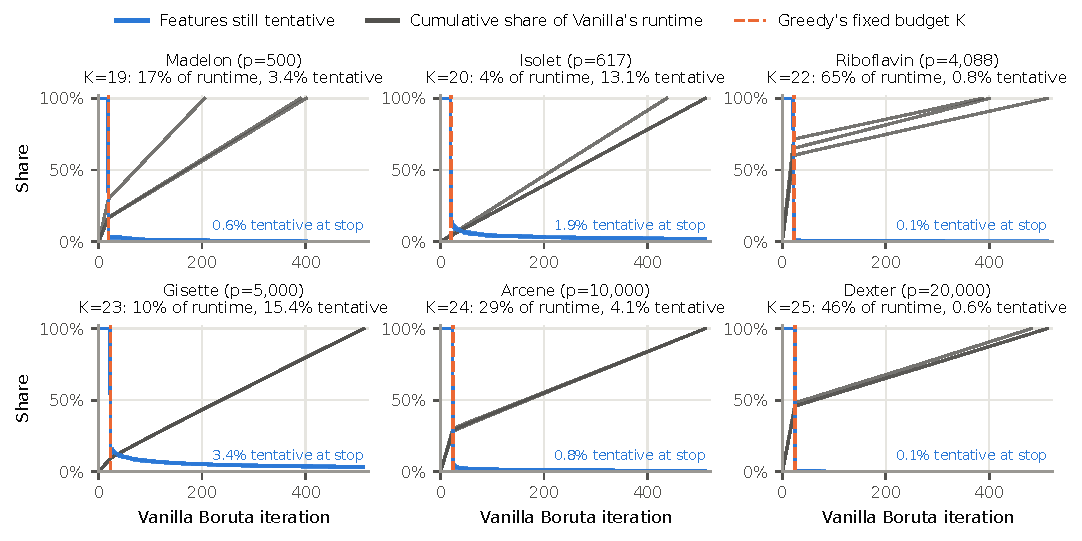
\includegraphics[width=\textwidth]{figures_v4/fig_runtime_anatomy.pdf}
  \caption{Anatomy of Vanilla Boruta runs ($\alpha=10^{-3}$, three folds per dataset). Blue: share of features still tentative; gray: cumulative share of the run's wall-clock time; dashed: Greedy Boruta's fixed budget $K$. Panel titles give both quantities at iteration $K$.}
  \label{fig:runtime_anatomy}
\end{figure}

\paragraph{Speedup.} This share determines the speedup (Fig.~\ref{fig:speedup}). The ratio of iterations, $12.8$--$39.4$ across datasets and $\alpha$, overstates the gain: Vanilla's later iterations are much cheaper than its first $K$, because rejected features leave the augmented matrix and the automatic tree count shrinks with them, whereas Greedy Boruta keeps all $p$ features in every iteration. Stopping Vanilla's own computation at iteration $K$ would yield $1.5\times$ (Riboflavin) to $25\times$ (Isolet), and serial Greedy Boruta achieves exactly this: its observed speedup is within $4\%$ of that bound on five of the six datasets (Madelon: $4.6\times$ against $5.9\times$). Iteration-level parallelism adds a further $1.1$--$3.9\times$, for median speedups of $1.7\times$ (Riboflavin) to $57\times$ (Isolet) at $\alpha=10^{-3}$, and up to $80\times$ at $\alpha=10^{-1}$. Serial Greedy Boruta also uses $1.1$--$25\times$ fewer CPU-seconds than Vanilla, so its gain is a reduction in work and not merely better core utilisation. Parallel execution has a memory cost, since each worker holds its own augmented matrix: the sampled peak memory increase reached $16$\,GB on Dexter, against $2$\,GB for Vanilla and serial Greedy Boruta.

\begin{figure}[H]
  \centering
  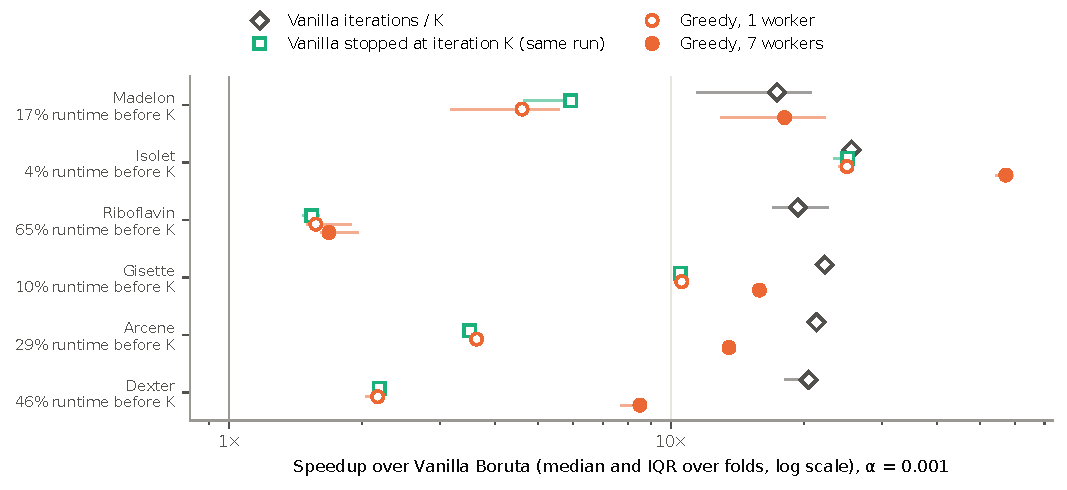
\includegraphics[width=\textwidth]{figures_v4/fig_speedup.pdf}
  \caption{Speedup over Vanilla Boruta (median and IQR over $15$ folds; $\alpha=10^{-3}$). Diamonds: Vanilla iterations$/K$; squares: Vanilla's own run stopped at iteration $K$ (three refits); circles: observed serial (open) and parallel (filled, $7$ workers) Greedy Boruta. Row labels give the share of Vanilla's runtime spent before iteration $K$.}
  \label{fig:speedup}
\end{figure}

\subsection{Selection Quality Against Ground Truth}
\label{sec:experiments:groundtruth}

\paragraph{Recall.} Greedy and Vanilla Boruta recover all $25$ relevant features in every fold of the reference and $p=2{,}000$ scenarios. With weak signal, both find about a third of them (Greedy: $0.34$, Vanilla rough fix: $0.34$, Vanilla strict: $0.32$ at $\alpha=10^{-3}$). In the coupled runs, Vanilla's strict and rough-fix selections are subsets of Greedy Boruta's in all $495$ fold--$\alpha$ combinations, as Theorem~\ref{thm:recall} requires.

\paragraph{False positives.} Fig.~\ref{fig:fp_bound} compares the mean number of false positives per fold with the bound $m_0K/(p+1)$ of Theorem~\ref{thm:fpr}. Greedy Boruta stays at $22$--$50\%$ of the bound in every scenario and at every $\alpha$, and the false positives grow much more slowly than $K$. The per-feature false positive rate falls from about $1.1\%$ at $p=500$ to $0.45\%$ at $p=2{,}000$, as the bound predicts. The gap to Vanilla Boruta is far smaller than the idealised comparison in Appendix~\ref{app:proofs} suggests. In the null scenario, where every selection is false, Vanilla confirms $4.7$ (strict) and $5.0$ (rough fix) noise features per fold against Greedy Boruta's $5.5$; only with strong signal (reference) does Vanilla select noticeably fewer ($1.7$ strict, $2.9$ rough fix, against $5.0$). The reason is that the data are fixed across iterations: a noise feature with a chance association to the target in the training sample beats the shadows repeatedly, violating the independence across iterations behind Vanilla's near-zero theoretical false positive rate. Such features are confirmed by both methods; Vanilla merely needs more iterations to do so.

\begin{figure}[H]
  \centering
  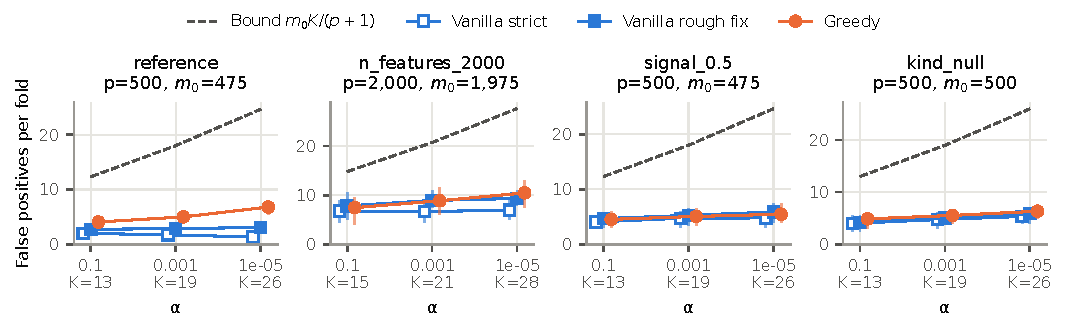
\includegraphics[width=\textwidth]{figures_v4/fig_fp_vs_bound.pdf}\\[2pt]
  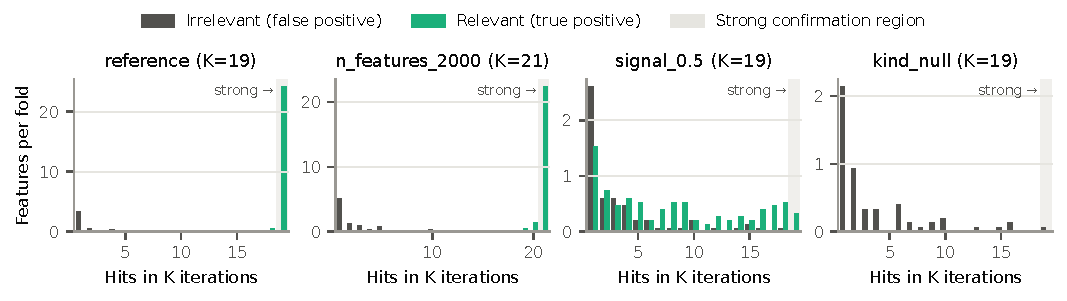
\includegraphics[width=\textwidth]{figures_v4/fig_hits.pdf}
  \caption{Top: false positives per fold against $\alpha$ (mean and IQR) with the bound $m_0K/(p+1)$. Bottom: hits within $K$ iterations of the features selected by coupled Greedy Boruta ($\alpha=10^{-3}$), per fold; the shaded region is the strong-confirmation range.}
  \label{fig:fp_bound}
\end{figure}

\paragraph{Weak and strong confirmations.} The hit counts in Fig.~\ref{fig:fp_bound} (bottom) separate the two kinds of selection. With strong signal, relevant features obtain a hit in essentially every iteration and are strongly confirmed, whereas false positives typically obtain one or two hits ($63\%$ have at most two). Across scenarios and $\alpha$, $98$--$100\%$ of Greedy Boruta's false positives are weak confirmations. With weak signal, relevant features also spread over low hit counts, and the weak set contains true and false positives in comparable numbers, which is exactly the population that the weak label flags for further scrutiny.

\subsection{Real-World Benchmarks}
\label{sec:experiments:realworld}

\paragraph{What Greedy Boruta adds.} Fig.~\ref{fig:fates} decomposes each coupled Greedy selection by Vanilla Boruta's outcome. Vanilla's final selection makes up $84$--$97\%$ of Greedy Boruta's on four datasets, $76\%$ on Gisette and $45\%$ on Arcene. Strong confirmations, which Vanilla makes at iteration $K$, range from $87\%$ of the selection (Isolet) to almost none (Arcene, with $160$ training samples). The remaining weak confirmations are mostly features that Vanilla Boruta also confirms, only later. In the refitted runs, Vanilla confirmed $66$--$71\%$ of Greedy's weak features on Madelon, Isolet, Riboflavin and Dexter, and decided them at a median iteration of $39$--$74$, two to three times $K$. On Gisette and Arcene, about half of the weak features are eventually rejected. These are the features that make Greedy Boruta's selection larger (Gisette: $2{,}035$ against $1{,}547$; Arcene: $420$ against $187$).

\begin{figure}[H]
  \centering
  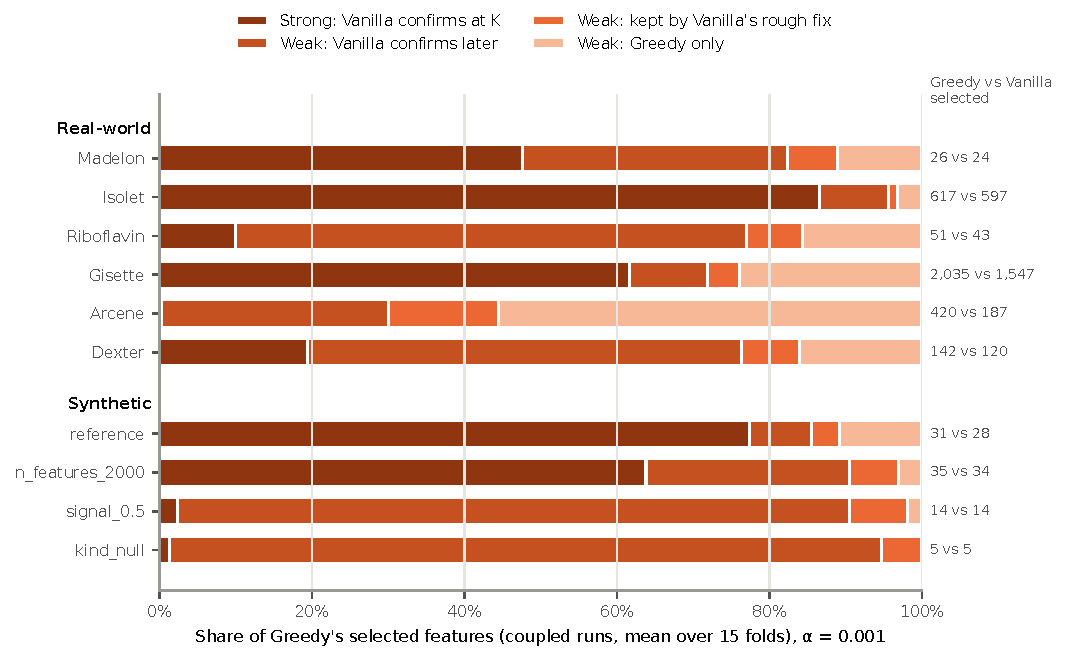
\includegraphics[width=\textwidth]{figures_v4/fig_greedy_fates.pdf}
  \caption{Composition of coupled Greedy Boruta selections by Vanilla Boruta's outcome ($\alpha=10^{-3}$, mean over $15$ folds). Strong confirmations are exactly Vanilla's confirmations at iteration $K$; the other layers are weak confirmations that Vanilla confirms later, keeps through the rough fix, or does not select.}
  \label{fig:fates}
\end{figure}

\paragraph{Downstream performance.} Table~\ref{tab:realworld_results} and Fig.~\ref{fig:ni} report the paired comparison. The mean score difference lies within the $0.01$ margin, or favours Greedy Boruta, in $17$ of the $18$ dataset--$\alpha$ combinations; the exception is Riboflavin at $\alpha=10^{-5}$ ($-0.012$ in $R^2$, with a fold standard deviation of about $0.2$). Non-inferiority is established on Gisette and Isolet at every $\alpha$ and is inconclusive on the other four datasets, also at the sensitivity level $0.025$. This reflects the resolution of the test rather than a difference between the methods: with $15$ overlapping folds the corrected standard error is three to five times the margin on the small datasets (Arcene, Riboflavin), and the all-feature model, which performs no selection at all, passes or fails in exactly the same places. Coupling the random streams reduces the standard deviation of the paired differences by $10$--$50\%$. Finally, $\alpha$ has little influence beyond the iteration budget (Fig.~\ref{fig:alpha}): smaller $\alpha$ lowers the speedup moderately through a larger $K$, while selection sizes and score differences barely change.

% TABLE: tables/real_results_focus.tex (tab:realworld_results); all-alpha version -> appendix

\begin{figure}[H]
  \centering
  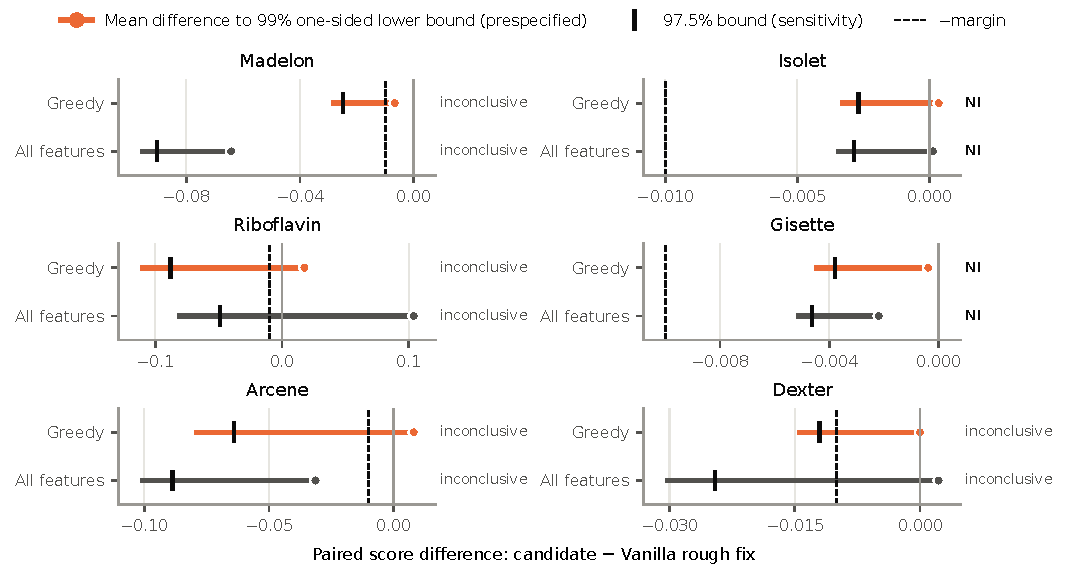
\includegraphics[width=\textwidth]{figures_v4/fig_noninferiority.pdf}
  \caption{Paired score difference with Vanilla Boruta ($\alpha=10^{-3}$): mean (dot), prespecified $99\%$ one-sided lower bound (end of bar), $97.5\%$ sensitivity bound (tick) and non-inferiority margin (dashed). The all-feature model calibrates the test.}
  \label{fig:ni}
\end{figure}

\begin{figure}[H]
  \centering
  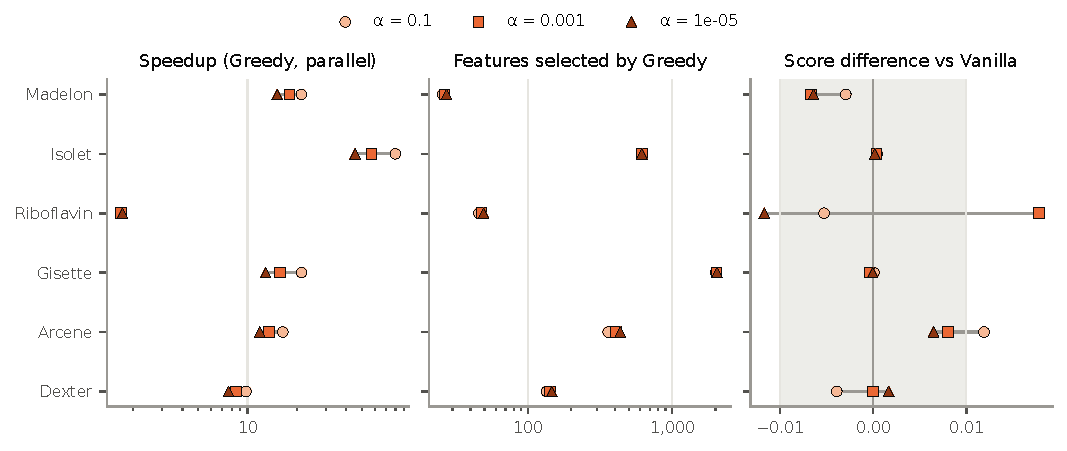
\includegraphics[width=\textwidth]{figures_v4/fig_alpha_sensitivity.pdf}
  \caption{Sensitivity to $\alpha$: parallel speedup, number of selected features and score difference with Vanilla Boruta (shaded: non-inferiority margin), one marker per $\alpha$.}
  \label{fig:alpha}
\end{figure}

\section{Discussion}
\label{sec:discussion}

\subsection{The Price of the Single-Hit Rule in Practice}
\label{sec:discussion:tradeoff}

Under idealised assumptions, Greedy Boruta exchanges a vanishing false positive rate for one bounded by $K/(p+1)$ (Theorem~\ref{thm:fpr}, Appendix~\ref{app:proofs}). The experiments show that the conservatism Vanilla Boruta buys is much smaller in practice. Its near-zero rate assumes that a noise feature's hits are independent across iterations, but all iterations share the same training data, so a feature with a chance association in the sample keeps beating the shadows. Vanilla then confirms it too, only later: in the null scenario it confirms $95\%$ of the noise features that Greedy Boruta selects. Greedy Boruta's additional false positives are few, remain well below the bound, decrease with $p$, and are almost all weak confirmations with one or two hits.

What Vanilla Boruta's extra iterations do buy is a decision on the small set of borderline features left at iteration $K$. Most of these are eventually confirmed; on Gisette and Arcene, about half are rejected, and there Greedy Boruta's selection is markedly larger. Combined with the weak/strong split, this suggests a practical workflow: use Greedy Boruta to resolve all features quickly, and direct further scrutiny, such as stability analysis, domain review or a longer Vanilla run restricted to these features, at the weak confirmations only.

\subsection{Limitations}
\label{sec:discussion:limitations}

\begin{enumerate}
  \item The FPR bound relies on shadow exchangeability (Assumption~\ref{asm:exchangeability}). Importance biases (e.g.\ towards high-cardinality features) affect both methods, but features with occasional, non-significant hits are confirmed weakly by Greedy Boruta and may remain tentative or be rejected by Vanilla Boruta.
  \item Speedups depend on how Vanilla Boruta distributes its work. When most features are rejected at iteration $K$ and the remaining iterations are cheap (Riboflavin, Dexter), the gain of serial Greedy Boruta is modest; parallel execution recovers much of it at the cost of memory proportional to the number of workers.
  \item The predictive comparison has limited resolution on small datasets: with $15$ overlapping folds, non-inferiority at a $0.01$ margin could not be established even for the all-feature model. The synthetic results come from a single realisation of each scenario.
  \item Both methods inherit the limitations of the base importance measure. With a pure XOR target, whose two relevant features are marginally uninformative, neither method nor the downstream model on all features detects the signal (Appendix~\ref{app:extra_results}).
\end{enumerate}


\section{Conclusion}
\label{sec:conclusion}

We have presented Greedy Boruta, a modification to the Boruta algorithm that replaces the binomial-test confirmation criterion with a single-hit rule: a feature is confirmed if it exceeds the maximum shadow importance in at least one iteration. This modification yields four formal guarantees: a conditional feature recall guarantee relative to Vanilla Boruta (Theorem~\ref{thm:recall}), convergence in exactly $K=\lceil \log_2(p/\alpha)\rceil$ iterations under Bonferroni correction (Theorem~\ref{thm:convergence}), a per-feature false positive rate bounded above by $K/(p+1)$ (Theorem~\ref{thm:fpr}) and the simplification of the final BH rejection calculation (Corollary~\ref{cor:bh}). As a consequence, Greedy Boruta eliminates all termination-related hyperparameters and substantially simplifies the multiple-testing correction framework used by Boruta.

Beyond the core algorithm, we introduced two practical extensions. First, we proposed a weak/strong confirmation framework that distinguishes features satisfying the original Boruta confirmation criterion from those selected exclusively by the greedy criterion, providing users with an interpretable measure of confidence among the confirmed features. Second, in Appendix \ref{app:add_results_reducing_shadows}, we showed that the number of shadow features can be reduced from $p$ to $r \leq p$, yielding an explicit trade-off between computational efficiency and false positive control. This extension is particularly attractive in high-dimensional and distributed computing environments, where the creation and storage of shadow features can become a substantial computational bottleneck.

Experiments on a synthetic benchmark with known ground truth and six real-world high-dimensional datasets support the theoretical analysis and demonstrate substantial computational gains, with speedups ranging from $1.8$ to $66.2\times$ while maintaining downstream predictive performance that is not detectably different from Vanilla Boruta in most configurations under the reported tests; this does not establish predictive equivalence.

We recommend Greedy Boruta as a practical default for all-relevant feature selection when downstream filtering, regularization or model validation procedures are available. The method is particularly appealing in high-dimensional settings, where its false positive rate remains small while its computational advantages become most pronounced. Future work includes extending the greedy criterion to alternative feature-importance measures, such as SHAP and permutation importance, and investigating the statistical properties of weakly confirmed features in large-scale applications. An open-source implementation is publicly available through the \texttt{greedyboruta} package on PyPI.

% =============================================================================
% ACKNOWLEDGMENTS (for camera-ready only)
% =============================================================================
% \paragraph{Acknowledgments.} We thank [names] for helpful discussions.

% =============================================================================
% REFERENCES
% =============================================================================

\bibliographystyle{splncs04}
\bibliography{references}

\appendix
\renewcommand{\theHsection}{\Alph{section}}

\section{Proofs}
\label{app:proofs}

For each feature $j$, define the total number of hits across $K$ iterations as
\[
H_j = \sum_{i=1}^{K} \mathbf{1}\!\left\{ I_j^{(i)} > M^{(i)} \right\},
\]
where $I_j^{(i)}$ denotes the importance of feature $j$ at iteration $i$ and $M^{(i)} = \max_j S_j^{(i)}$ denotes the maximum shadow importance at iteration $i$.

\subsection{Proof of Theorem~\ref{thm:recall} (Recall Guarantee)}

\begin{proof}
Let $H_j(K)$ count hits through Greedy Boruta's terminal iteration $K$. If $H_j(K)=0$, feature $j$ cannot have been confirmed by a binomial test through $K$, since its confirmation p-value is 1. Since Vanilla Boruta applies the same rejection test at iteration $K$, its rejection p-value there is $2^{-K}\leq\alpha/p$ under Bonferroni correction (or $2^{-K}\leq\alpha$ without it). Vanilla therefore rejects it by $K$ if it has not already been rejected.

Because rejections are final, feature $j$ cannot be confirmed later, either by a binomial test or by the rough fix, which only considers tentative features. Consequently, every feature confirmed at Vanilla's terminal iteration $T\geq K$ must have $H_j(K)\geq1$. The shared importance trajectory ensures that Greedy Boruta also observes that hit and selects $j$ at $K$. Therefore $\mathcal{C}_V(T)\subseteq\mathcal{C}_G(K)$; the terminal iteration counts need not be equal.
\end{proof}

\subsection{Proof of Theorem~\ref{thm:convergence} (Convergence Guarantee)}

\begin{proof}
At iteration $K$, partition the features into
$$
\mathcal{H}^{+} = \{j : H_j \geq 1\}
\quad\text{and}\quad
\mathcal{H}^{0} = \{j : H_j = 0\}.
$$
By Algorithm~\ref{alg:greedy_boruta} (line~14), all features in $\mathcal{H}^{+}$ are confirmed by Greedy Boruta. In contrast, for any feature $j \in \mathcal{H}^{0}$, the rejection test evaluates
$$
H_0 : p_j \geq 0.5
\quad \text{versus} \quad
H_1 : p_j < 0.5,
$$
where $p_j$ denotes the probability that feature $j$ exceeds the maximum shadow importance in a given iteration. Under the null hypothesis, the hit count follows
$$
H_j \sim \mathsf{Binomial}(K,\theta=0.5).
$$
Since $H_j = 0$, the rejection p-value is
$$
\mathbb{P}(H_j = 0 \mid K,\theta=0.5)
=
(0.5)^K
=
2^{-K}.
$$
Notice that all features in $\mathcal{H}^0$ have this identical p-value. Under Bonferroni correction across $|\mathcal{H}^0| \leq p$ features, rejection requires $2^{-K} \leq \alpha/p$. The minimum integer satisfying this is $K = \lceil \log_2(p/\alpha) \rceil$. In practice, at iteration $K$ all features in $\mathcal{H}^0$ are rejected and all in $\mathcal{H}^+$ are confirmed, so the algorithm terminates with no tentative features.
\end{proof}
\noindent
\textit{Note}: Without Bonferroni correction, rejection requires $2^{-K} \leq \alpha$, giving $K = \lceil \log_2(1/\alpha) \rceil$. 

\subsection{Proof of Corollary~\ref{cor:bh} (BH Rejection Simplification)}

\begin{proof}
From the proof of Theorem~\ref{thm:convergence}, any tentative feature $j$ at iteration $K$ has $H_j = 0$ and p-value $p^* = 2^{-K}$.

The Benjamini-Hochberg procedure orders p-values $p_{(1)} \leq \cdots \leq p_{(m)}$ and finds the largest $i$ such that $p_{(i)} \leq (i/m) \cdot \alpha$. Since all p-values are identical ($p_{(i)} = p^*$ for all $i$), this reduces to checking whether $p^* \leq \alpha$. Under either correction setting, $K \geq \lceil \log_2(1/\alpha) \rceil$, so $p^* = 2^{-K} \leq \alpha$ and the condition holds at $i = m$ and all tentative features are rejected. Hence, the FDR-corrected and uncorrected procedures coincide.
\end{proof}

\subsection{Proof of Theorem~\ref{thm:fpr} (FPR of Greedy Boruta)}

\begin{proof}
For an irrelevant feature $j$, let $A_i=\{I_j^{(i)}>M^{(i)}\}$ denote a hit in iteration $i$. Under Assumption~\ref{asm:exchangeability}, each of the $p+1$ importances has the same probability of being the unique maximum. These events are disjoint, so $\mathbb{P}(A_i)\leq 1/(p+1)$, with equality if the maximum is unique almost surely. A false confirmation occurs if at least one $A_i$ occurs. The union bound gives
\[
\mathbb{P}\!\left(\bigcup_{i=1}^{K} A_i\right)
\leq \sum_{i=1}^{K}\mathbb{P}(A_i)
\leq \frac{K}{p+1}.
\]
This bound allows ties and does not require independence across iterations. Under the additional assumptions of independent hit events across iterations and an almost surely unique maximum in every iteration, the exact probability is $1-(p/(p+1))^K$, which the bound above dominates.

For the expected number of false positives, let $\mathcal{N}$ be the set of $m_0$ irrelevant features. By linearity of expectation, which holds for dependent random variables,
\[
\mathbb{E}[\mathrm{FP}] = \sum_{j\in\mathcal{N}} \mathbb{P}(j \text{ is confirmed}) \leq \frac{m_0 K}{p+1}.
\]
\end{proof}

\paragraph{Comparison with Vanilla Boruta.}
Under Assumption~\ref{asm:exchangeability}, the FPR of Vanilla Boruta is effectively negligible. In Vanilla Boruta, without Bonferroni correction, a feature is confirmed only if its hit count exceeds a threshold \(h^*\) satisfying
\[
\mathbb{P}(\mathsf{Binomial}(K,\theta=0.5) \geq h^*) \leq \alpha.
\]
For the following idealized fixed-horizon comparison, assume independent hit events across iterations and an almost surely unique maximum in addition to exchangeability. Then the per-iteration hit probability is \(\theta_0 = 1/(p+1)\), and its hit count follows
\[
H_j \sim \mathsf{Binomial}(K,\theta_0).
\]
Consequently, the probability that an irrelevant feature is falsely confirmed by Vanilla Boruta is $\mathbb{P}(H_j \geq h^*)$, which decays exponentially in \(K\) and is therefore extremely small in high-dimensional settings. For example, with \(\alpha = 0.001\) and \(p = 500\), Greedy Boruta requires \(K = 19\) iterations, while Vanilla Boruta requires at least \(h^* = 19\) hits for confirmation. Under the null hit probability \(\theta_0 = 1/501\), the resulting false positive probability for Vanilla Boruta is approximately \(10^{-52}\), compared to the false positive probability under Greedy Boruta
\[
\mathbb{P}(H_j \geq 1)
=
1 - \left(\frac{500}{501}\right)^{19}
\approx 3.73\%.
\]
This contrast reflects the central trade-off between the two procedures: Greedy Boruta sacrifices the near-zero FPR of Vanilla Boruta in exchange for deterministic convergence, elimination of tentative features, and substantially improved computational efficiency.

% \subsection{Proof of Proposition~\ref{prop:mr_mp}}

% \begin{proof}
% The event \(\{M_r = M_p\}\) occurs if, and only if, all of the remaining \(p-r\) variables are smaller than \(M_r\). Conditioning on \(M_r\),
% \[
% \mathbb{P}(M_r = M_p \mid M_r)
% =
% F(M_r)^{p-r}.
% \]
% Taking the expectation yields
% \[
% \mathbb{P}(M_r = M_p)
% =
% \mathbb{E}\!\left[F(M_r)^{p-r}\right].
% \]
% We now derive the distribution of \(F(M_r)\). For any \(u \in [0,1]\),
% \begin{align*}
% \mathbb{P}(F(M_r) \leq u)
% &=
% \mathbb{P}(M_r \leq F^{-1}(u)) \\
% &=
% \mathbb{P}(S_1 \leq F^{-1}(u),\ldots,S_r \leq F^{-1}(u)) \\
% &=
% \prod_{i=1}^{r} \mathbb{P}(S_i \leq F^{-1}(u)) \\
% &=
% u^r.
% \end{align*}
% Therefore,
% \[
% F(M_r) \sim \mathrm{Beta}(r,1),
% \]
% with density
% \[
% f(u)=r\,u^{r-1},
% \qquad 0 \leq u \leq 1.
% \]
% Consequently,
% \begin{align*}
% \mathbb{P}(M_r = M_p)
% &=
% \mathbb{E}\!\left[F(M_r)^{p-r}\right] \\
% &=
% \int_0^1 u^{p-r} \, r u^{r-1}\,du \\
% &=
% r\int_0^1 u^{p-1}\,du \\
% &=
% \frac{r}{p}.
% \end{align*}
% \end{proof}

\section{Reducing the Number of Shadow Features}
\label{app:add_results_reducing_shadows}

By relaxing the confirmation criterion for relevant features while preserving the statistical rigour of the rejection criterion, Greedy Boruta achieves substantial reductions in computational time across the datasets considered in Section~\ref{sec:experiments}. A key advantage of Greedy Boruta is that the total number of iterations can be determined analytically from the significance level~\(\alpha\) and the number of features $p$, unlike Vanilla Boruta, whose convergence behavior depends on sequential hypothesis testing and heuristic stopping rules. In this section, we further investigate how the computational cost of Greedy Boruta can be reduced by decreasing the number of shadow features used to define the random-noise threshold at each iteration. We refer to this variant as \textit{reduced-shadow} Greedy Boruta.

% To quantify the effect of using only $r$ shadow features, we first establish the following result, which the proof is given in Appendix~\ref{app:proofs}.

% \begin{proposition}
% \label{prop:mr_mp}
% Let \(S_1,\ldots,S_p\) be i.i.d.\ continuous random variables denoting shadow importances with cumulative distribution function \(F\). Define
% \[
% M_r = \max(S_1,\ldots,S_r),
% \qquad
% M_p = \max(S_1,\ldots,S_p),
% \]
% for \(r \leq p\). Then
% \[
% \mathbb{P}(M_r = M_p) = \frac{r}{p}.
% \]
% \end{proposition}
% \begin{remark}
% The result above quantifies how often the reduced-shadow threshold coincides exactly with the threshold that would have been obtained using all $p$ shadows. In practice, the reduced-shadow threshold agrees with the one from vanilla Boruta with probability $r/p$.
% \end{remark}

% \begin{remark}
% The result also follows immediately from symmetry. Among the \(p\) shadow importances, the global maximum $M_p$ is equally likely to occur at any index. Therefore, the probability that the global maximum belongs to the subset of size \(r\) is \(r/p\).
% \end{remark}


% Recall that both Vanilla Boruta and Greedy Boruta augment the original dataset containing \(p\) features with \(p\) shadow features obtained through random permutations of the original covariates. Consequently, as shown in Algorithm~\ref{alg:greedy_boruta}, the base estimator is trained on a design matrix of dimension \(n \times 2p\). However, when \(p\) is large, constructing all \(p\) shadow features may become computationally expensive. To address this, we consider using only \(r \leq p\) shadow features instead of the full set of \(p\) shadows. In practice, at each iteration, we generate only $r$ shadow features obtained by randomly permuting $r$ selected covariates. The random-noise threshold is defined as the maximum importance among the generated shadow features. This modification is particularly attractive in high-dimensional settings, where the cost of fitting the base estimator dominates the overall runtime. In addition, this may be important when shadow feature creation and storage is most costly, for example, when the augmented dataset does not fully fit in RAM and overhead regarding materializing to disk is added.

Recall that both Vanilla Boruta and Greedy Boruta augment the original dataset containing \(p\) features with \(p\) shadow features obtained through random permutations of the original covariates. Consequently, as shown in Algorithm~\ref{alg:greedy_boruta}, the base estimator is trained on a design matrix of dimension \(n \times 2p\). However, when \(p\) is large, constructing all \(p\) shadow features may become computationally expensive. To address this, we consider using only \(r \leq p\) shadow features instead of the full set of \(p\) shadows. In practice, at each iteration, we generate only \(r\) shadow features obtained by randomly permuting \(r\) selected covariates. The random-noise threshold is then defined as the maximum importance among the generated shadow features.

This modification is particularly attractive in high-dimensional settings, where the cost of fitting the base estimator dominates the overall runtime. Moreover, reducing the number of shadow features can substantially decrease memory and storage requirements. This is especially relevant in distributed computing environments for big data, such as Apache Spark \cite{zaharia2016spark}, where the augmented dataset may not fit entirely in memory. In such settings, shadow features either need to be represented explicitly in the execution plan or materialized as intermediate data on disk, both of which introduce additional computational and storage overhead. Using fewer shadow features alleviates these costs while preserving the statistical framework of the method.

% As discussed in Section~\ref{sec:method:fpr}, under Assumption~\ref{asm:exchangeability}, the importance of an irrelevant feature and the \(p\) shadow importances form \(p+1\) exchangeable random variables. Consequently, when all \(p\) shadow features are used, each variable is equally likely to attain the maximum importance score, implying that the per-iteration hit probability of an irrelevant feature is
% \[
% \theta_0 = \frac{1}{p+1}.
% \]


% Assume $S_1,\dots,S_p$ are i.i.d. continuous random variables denoting shadow feature importances with cumulative distribution function \(F\), and define
% $$
% M_p = \max_{1 \leq j \leq p} S_j,
% \qquad
% M_r = \max_{1 \leq j \leq r} S_j.
% $$
% Conditioning on the observed shadow importances,
% \[
% \mathbb{P}(M_r=M_p \mid S_1,\ldots,S_r)
% =
% F(M_r)^{p-r},
% \]
% since all remaining \(p-r\) shadow importances must fall below \(M_r\).

% \begin{enumerate}
%     \item For any \textit{observed importance} \(i \leq r\),
% $$
% \mathbb{P}(S_i = M_p \mid S_1,\dots,S_r)
% =
% \mathbf{1}\{S_i = M_r\}\,F(S_i)^{p-r}.
% $$
% That is, if \(S_i \neq M_r\), then \(S_i\) cannot be the global maximum. Otherwise, if \(S_i = M_r\), then all remaining \(p-r\) variables must satisfy $S_{r+1},\dots,S_p < S_i$, which occurs with probability \(F(S_i)^{p-r}\). \\


% \item For any \textit{unobserved importance} \(i > r\),
% $$
% \mathbb{P}(S_i = M_p \mid S_1,\dots,S_r)
% =
% \int_{M_r}^{\infty} F(x)^{p-r-1}\,dF(x).
% $$
% Using the substitution \(u = F(x)\),
% \begin{align}
% \mathbb{P}(S_i = M_p \mid S_1,\dots,S_r) & = \int_{F(M_r)}^{1} u^{p-r-1}\,du \nonumber \\
% & = \frac{1 - F(M_r)^{p-r}}{p-r} \nonumber.
% \end{align}
% Summing over $p-r$ unobserved shadows gives
% $$
% 1 - F(M_r)^{p-r},
% $$
% which is the probability that some unseen shadow exceeds $M_r$. Therefore, $F(M_r)^{p-r}$ is the probability that the maximum among the sampled shadows is also the global shadow maximum (i.e., $M_r = M_p)$.
% \end{enumerate}
Let \(\theta_0^\star\) denote the per-iteration hit probability of an irrelevant feature when only \(r\) shadow features are used. Under Assumption~\ref{asm:exchangeability} for these \(r+1\) importances,
\[
\theta_0^\star \leq \frac{1}{r+1},
\]
with equality when the maximum is unique almost surely. Applying the union-bound argument from Theorem~\ref{thm:fpr} gives
\begin{align}
\label{eqn:fpr_upper_bound}
\mathbb{P}(H_j \geq 1)
&\leq \sum_{i=1}^{K}\mathbb{P}\!\left(I_j^{(i)}>M_r^{(i)}\right) \nonumber\\
&\leq \frac{K}{r+1},
\end{align}
where $M_r^{(i)}$ is the maximum importance among the $r$ shadows in iteration $i$. With the additional assumptions of independent hit events across iterations and an almost surely unique maximum, the exact probability is $1-(1-1/(r+1))^K$.
This result highlights a direct trade-off between computational cost and false positive control. Reducing the number of shadow features decreases the dimensionality of the augmented design matrix from \(2p\) to \(p+r\), potentially yielding substantial computational savings. However, the upper bound on the null hit probability increases from \(1/(p+1)\) to \(1/(r+1)\), weakening the FPR guarantee.

Under these additional assumptions, Figure~\ref{fig:relative_fpr_shadows} illustrates this trade-off for different combinations of number of features \(p\), significance level \(\alpha\) and fraction of shadow features \(r/p\). The impact of reducing the number of shadow features depends strongly on the dimensionality of the problem. For small values of \(p\), the FPR is already relatively large when all shadow features are used, so further reductions in \(r\) may lead to an undesirable increase in spurious confirmations. For example, when \(p=500\) and \(\alpha=0.05\), the per-feature FPR is approximately \(2.8\%\) when \(r=p\) and increases $4.6$ times to \(13\%\) when only \(20\%\) of the shadow features are used. In contrast, for moderate and large values of \(p\), the FPR remains small even when only a fraction of the shadow features is used. For instance, when \(p=10{,}000\) and \(\alpha=0.05\), the FPR is approximately \(0.18\%\) when \(r=p\) and remains below \(1\%\) when only \(20\%\) of the shadow features are used. In practice, an FPR of \(\gamma\) indicates that a truly irrelevant feature is incorrectly confirmed with probability \(\gamma\). Therefore, if there are \(m_0\) irrelevant features, the expected number of false positives is \(m_0\gamma\).

\begin{figure}
    \centering
    \includegraphics[width=\linewidth]{relative_FPR_with_shadows.png}
    \caption{Per-feature false positive rate (FPR) relative to the minimum FPR across all $\alpha$ at $100\%$ of Greedy Boruta under Bonferroni correction using different number of features, fraction of shadow features and significance level.}
    \label{fig:relative_fpr_shadows}    
\end{figure}

A practical question is how to choose the number of shadow features \(r\). Given the upper bound on the FPR in Equation \eqref{eqn:fpr_upper_bound}, one could, in principle, select \(r\) so that the upper bound does not exceed a significance level \(\alpha\). Solving
\[
\frac{K}{r+1}\leq \alpha
\]
yields the condition $r \geq K/\alpha-1$. Therefore, define the minimum required shadow count as
\[
r_{\min}=\left\lceil \frac{K}{\alpha}-1\right\rceil.
\]
Choose $r=r_{\min}$ only when $1\leq r_{\min}\leq p$ (or $r=1$ if $r_{\min}<1$). If $r_{\min}>p$, no $r\leq p$ can certify the target using this bound. Clipping $r_{\min}$ to $p$ does not preserve the guarantee. This is a feasibility limitation of the bound, not a proof that the actual FPR exceeds the target.

% Finally, Figure~\ref{fig:fpr_shadows} and Table~\ref{tab:fpr_shadows_exact} report the theoretical FPR for different combinations of the number of features \(p\), the fraction of shadow features \(r/p\) and the significance level \(\alpha\).

% \begin{figure}[H]
%     \centering
%     \includegraphics[width=\linewidth]{FPR_with_shadows.png}
%     \caption{Exact per-feature false positive rate (FPR) of Greedy Boruta under Bonferroni correction using different number of features, fraction of shadow features and significance level.}
%     \label{fig:fpr_shadows}
% \end{figure}

% \begin{table}[H]
% \centering
% \caption{Exact per-feature false positive rate (FPR) of Greedy Boruta under Bonferroni correction using different numbers of features, fractions of shadow features, and significance levels. The FPR is computed as $1-(1-\frac{1}{r+1})^K$, where $K=\lceil \log_2(p/\alpha)\rceil$.}
% \label{tab:fpr_shadows_exact}

% \begin{subtable}{\textwidth}
% \centering
% \caption{$r = 0.10p$}
% \begin{tabular}{c|cc|cc|cc|cc}
% \toprule
% & \multicolumn{2}{c|}{$p = 100$}
% & \multicolumn{2}{c|}{$p = 500$}
% & \multicolumn{2}{c|}{$p = 1{,}000$}
% & \multicolumn{2}{c}{$p = 10{,}000$} \\
% $\alpha$
% & $K$ & FPR
% & $K$ & FPR
% & $K$ & FPR
% & $K$ & FPR \\
% \midrule
% $0.05$    & 11 & 64.95\% & 14 & 24.21\% & 15 & 13.87\% & 18 & 1.78\% \\
% $0.01$    & 14 & 73.67\% & 16 & 27.16\% & 17 & 15.56\% & 20 & 1.98\% \\
% $0.001$   & 17 & 80.22\% & 19 & 31.36\% & 20 & 18.05\% & 24 & 2.37\% \\
% $0.0001$  & 20 & 85.14\% & 23 & 36.58\% & 24 & 21.24\% & 27 & 2.66\% \\
% $0.00001$ & 24 & 89.85\% & 26 & 40.24\% & 27 & 23.56\% & 30 & 2.95\% \\
% \bottomrule
% \end{tabular}
% \end{subtable}

% % \vspace{0.3cm}

% \begin{subtable}{\textwidth}
% \centering
% \caption{$r = 0.25p$}
% \begin{tabular}{c|cc|cc|cc|cc}
% \toprule
% & \multicolumn{2}{c|}{$p = 100$}
% & \multicolumn{2}{c|}{$p = 500$}
% & \multicolumn{2}{c|}{$p = 1{,}000$}
% & \multicolumn{2}{c}{$p = 10{,}000$} \\
% $\alpha$
% & $K$ & FPR
% & $K$ & FPR
% & $K$ & FPR
% & $K$ & FPR \\
% \midrule
% $0.05$    & 11 & 35.04\% & 14 & 10.56\% & 15 & 5.81\% & 18 & 0.72\% \\
% $0.01$    & 14 & 42.25\% & 16 & 11.97\% & 17 & 6.56\% & 20 & 0.80\% \\
% $0.001$   & 17 & 48.66\% & 19 & 14.05\% & 20 & 7.67\% & 24 & 0.96\% \\
% $0.0001$  & 20 & 54.36\% & 23 & 16.75\% & 24 & 9.14\% & 27 & 1.07\% \\
% $0.00001$ & 24 & 60.99\% & 26 & 18.71\% & 27 & 10.22\% & 30 & 1.19\% \\
% \bottomrule
% \end{tabular}
% \end{subtable}

% % \vspace{0.3cm}

% \begin{subtable}{\textwidth}
% \centering
% \caption{$r = 0.50p$}
% \begin{tabular}{c|cc|cc|cc|cc}
% \toprule
% & \multicolumn{2}{c|}{$p = 100$}
% & \multicolumn{2}{c|}{$p = 500$}
% & \multicolumn{2}{c|}{$p = 1{,}000$}
% & \multicolumn{2}{c}{$p = 10{,}000$} \\
% $\alpha$
% & $K$ & FPR
% & $K$ & FPR
% & $K$ & FPR
% & $K$ & FPR \\
% \midrule
% $0.05$    & 11 & 19.57\% & 14 & 5.44\% & 15 & 2.95\% & 18 & 0.36\% \\
% $0.01$    & 14 & 24.21\% & 16 & 6.19\% & 17 & 3.34\% & 20 & 0.40\% \\
% $0.001$   & 17 & 28.58\% & 19 & 7.30\% & 20 & 3.92\% & 24 & 0.48\% \\
% $0.0001$  & 20 & 32.70\% & 23 & 8.77\% & 24 & 4.68\% & 27 & 0.54\% \\
% $0.00001$ & 24 & 37.83\% & 26 & 9.86\% & 27 & 5.25\% & 30 & 0.60\% \\
% \bottomrule
% \end{tabular}
% \end{subtable}

% % \vspace{0.3cm}

% \begin{subtable}{\textwidth}
% \centering
% \caption{$r = 0.75p$}
% \begin{tabular}{c|cc|cc|cc|cc}
% \toprule
% & \multicolumn{2}{c|}{$p = 100$}
% & \multicolumn{2}{c|}{$p = 500$}
% & \multicolumn{2}{c|}{$p = 1{,}000$}
% & \multicolumn{2}{c}{$p = 10{,}000$} \\
% $\alpha$
% & $K$ & FPR
% & $K$ & FPR
% & $K$ & FPR
% & $K$ & FPR \\
% \midrule
% $0.05$    & 11 & 13.56\% & 14 & 3.66\% & 15 & 1.98\% & 18 & 0.24\% \\
% $0.01$    & 14 & 16.93\% & 16 & 4.17\% & 17 & 2.24\% & 20 & 0.27\% \\
% $0.001$   & 17 & 20.16\% & 19 & 4.93\% & 20 & 2.63\% & 24 & 0.32\% \\
% $0.0001$  & 20 & 23.27\% & 23 & 5.94\% & 24 & 3.15\% & 27 & 0.36\% \\
% $0.00001$ & 24 & 27.23\% & 26 & 6.69\% & 27 & 3.53\% & 30 & 0.40\% \\
% \bottomrule
% \end{tabular}
% \end{subtable}

% % \vspace{0.3cm}

% \begin{subtable}{\textwidth}
% \centering
% \caption{$r = p$ (original Greedy Boruta)}
% \begin{tabular}{c|cc|cc|cc|cc}
% \toprule
% & \multicolumn{2}{c|}{$p = 100$}
% & \multicolumn{2}{c|}{$p = 500$}
% & \multicolumn{2}{c|}{$p = 1{,}000$}
% & \multicolumn{2}{c}{$p = 10{,}000$} \\
% $\alpha$
% & $K$ & FPR
% & $K$ & FPR
% & $K$ & FPR
% & $K$ & FPR \\
% \midrule
% $0.05$    & 11 & 10.37\% & 14 & 2.76\% & 15 & 1.49\% & 18 & 0.18\% \\
% $0.01$    & 14 & 13.00\% & 16 & 3.15\% & 17 & 1.68\% & 20 & 0.20\% \\
% $0.001$   & 17 & 15.56\% & 19 & 3.73\% & 20 & 1.98\% & 24 & 0.24\% \\
% $0.0001$  & 20 & 18.05\% & 23 & 4.49\% & 24 & 2.37\% & 27 & 0.27\% \\
% $0.00001$ & 24 & 21.24\% & 26 & 5.06\% & 27 & 2.66\% & 30 & 0.30\% \\
% \bottomrule
% \end{tabular}
% \end{subtable}

% \end{table}

\subsection{Reduced-Shadow Greedy Boruta on Real-World Benchmarks}


% #2 (reduced-shadow experiments on real data): worth doing, and cheap credibility. Take the four largest-pp
% p datasets (Dexter, Arcene, Gisette, Riboflavin), fix α=10−3\alpha=10^{-3}
% α=10−3 rather than sweeping, sweep r/p∈{0.1,0.25,1}r/p \in \{0.1, 0.25, 1\}
% r/p∈{0.1,0.25,1}, and report score, time, number confirmed (with the weak/strong split), with Vanilla as a reference column. One table plus a short paragraph in the style of the Downstream Performance section. On the files: the stats and table-generation code came from your side in the session where we built that section; I can pull together what we have from there and extend the runner with an r parameter whenever you want.


\end{document}

